\documentclass[subeqn]{article}

\title{The Twin Instrument\footnote{We are grateful to Paul Devereux, James 
    Fenske, Judith Hall, Cheti Nicoletti, Carol Propper, Margaret Stevens,
    Atheen Venkataramani, Marcos Vera-Hernandez, Frank Windmeijer,
    Emilia Del Bono, Climent Quintana-Domeque, Pedro R\'odenas, Libertad
    Gonz\'alez, Hanna M\"uhlrad, Anna Aevarsdottir, Martin Foureaux
    Koppensteiner, Ryan Palmer and Pietro Biroli along with various seminar
    audiences and discussants for helpful comments and/or sharing data. All
    remaining errors are our own.}}
\author{Sonia Bhalotra\thanks{Department of Economics and ISER, The University of
    Essex. Contact: \href{mailto:srbhal@essex.ac.uk}{srbhal@essex.ac.uk}} 
\and Damian Clarke\thanks{Deparment of Economics, Universidad de Santiago de Chile.
Contact: \href{mailto:damian.clarke@usach.cl}
{damian.clarke@economics.ox.ac.uk}}}
\date{August 11, 2016}

%at CMPO Bristol, ESPE, NEUDC, CSAE, The University of Essex, The University of 
%Oxford, the Barcelona GSE summer forum, PacDev, the RES conference, Germany,
%Essen, Other Sweden, University of Chile, University of Santiago de Chile

%*******************************************************************************
\usepackage{amsmath}
\usepackage{amssymb}
\usepackage{appendix}
\usepackage{blindtext}
\usepackage{bm}
\usepackage{booktabs}
\usepackage{breqn}
\usepackage{caption}
\usepackage[usenames, dvipsnames]{color} \pagecolor{white}
\usepackage{dcolumn}
\usepackage{epsfig}
\usepackage{epstopdf}
\usepackage[capposition=top]{floatrow}
\usepackage{hyperref}
\usepackage{lastpage}
\usepackage{longtable}
\usepackage{lscape}
\usepackage{multirow}
\usepackage{natbib} \bibliographystyle{abbrvnat}\bibpunct{(}{)}{;}{a}{,}{,}
\usepackage{pdfpages}
\usepackage{rotating}
\usepackage{setspace}
\usepackage{subcaption}
\usepackage{subfloat}
\usepackage{url}
\usepackage{wrapfig}
\usepackage{xr}
\externaldocument{onlineAppendix_Twins}

%*******************************************************************************
\setlength\topmargin{-0.375in}
\setlength\textheight{8.8in}
\setlength\textwidth{5.8in}
\setlength\oddsidemargin{0.4in}
\setlength\evensidemargin{-0.5in}
\setlength\parindent{0.25in}
\setlength\parskip{0.25in}

\hypersetup{
    colorlinks=true,   
    linkcolor=BlueViolet,
    citecolor=Black,
    filecolor=BlueViolet,
    urlcolor=BlueViolet
}


\newcommand{\twinfolder}{"/home/damian/investigacion/Activa/Twins"}
\DeclareMathOperator{\plim}{plim}

\renewcommand{\familydefault}{\sfdefault}
%*******************************************************************************
\begin{document}
\begin{spacing}{1.4}

\maketitle
\vspace{-1cm}
%\begin{center}{\Large\textsc{Preliminary Draft}}\end{center}
\begin{abstract}
 The incidence of twins has been used to identify the impact of changes in 
 fertility on measures of investment in children born prior to the twins, and
 the emerging consensus in this literature is that there is no evidence of a
 quantity-quality (Q--Q) trade-off. We argue that the standard approach is 
 flawed. Even if twin conception is random, bringing twins to term is a function 
 of maternal health which is difficult to fully observe and which tends to be
 correlated with child quality, rendering the instrument invalid. The neglect
 of this fact in the existing literature will tend to lead to under-estimation 
 of the Q--Q trade-off and so could contribute to explaining the negative results
 in the literature. Our contention that women who produce twin births are
 positively selected is demonstrated using data from richer and poorer countries.
 Using large samples of microdata from developing countries and from the USA 
 which include indicators of maternal health characteristics and behaviours, we
 show that a significant trade-off emerges upon correcting for these biases. We
 show that this result is likely to be only a \emph{lower} bound of the true
 Q--Q trade-off and discuss how to estimate the size of these bounds. These
 results have important implications for twin studies in all contexts examined
 here.
\\
\end{abstract}
\hspace{4mm}\textbf{\small JEL codes}: J12,J13,C13,D13,I12. \\

\newpage
%*******************************************************************************
\section*{Introduction}                             \label{TWINscn:intro}
Since the pioneering work of \citet{RosenzweigWolpin1980}, economists have 
attempted to leverage the occurrence of twin births to estimate the effect of 
family size on child outcomes. If twin births occur at random, their occurrence 
constitutes a fertility shock that is uncorrelated with family characteristics, 
including parental preferences, and other unobservables which may be related to 
child quality. This provides the exogenous variation (in quantity) required to 
estimate the quantity-quality model of \citet{Becker1960,BeckerLewis1973,
BeckerTomes1976}.  The essential idea of these studies is that the shadow price 
of child quality is increasing in child quality and \emph{vice versa}. Thus, by 
comparing those families who unexpectedly produced additional children with 
those who always produced one child per birth, it is argued that the effect of 
an additional sibling on a child's human capital attainment can be uniquely
identified.

However, the consistent estimation of this effect is based upon the untestable 
assumption that twinning is exogenous. This requires not only that twin 
conceptions are randomly assigned to families, but also that taking a twin
conception to term does not depend upon a woman's behaviours during pregnancy 
or on her endowments prior to pregnancy. This is at odds with the evidence.

We show that endowments and behaviours affect the chances of twins being born. 
In data from a large sample of developing countries, we show that taller women 
and women with a higher body-mass index are significantly more likely to give 
birth to twins.\footnote{Height is an index of the stock of health of a woman 
and is a function of investments over her growth period and, especially, the 
early years of her life (see references in \citet{BhalotraRawlings2013}).} 
Maternal health is likely to be an especially significant determinant of birth 
outcomes in poorer countries where many women are chronically under-nourished 
(an indicator of which is their final stature), exhibit anemia and low-BMI, and 
are prone to infections. In these conditions only relatively healthy women will 
have the resources to support a successful twin pregnancy. However, our critique 
applies to richer countries too. Using administrative data from the Scotland,
the USA, Sweden and Spain, and survey data from the UK and Chile, we find that 
women who are taller and less likely to engage in risky behaviours such as 
smoking, drug taking or alcohol consumption during pregnancy are significantly 
more likely to have a (live) twin birth \citep{BhalotraClarke2016}.\footnote{%
  Simiarly, it is well known 
that fertility treatments increase the likelihood of twinning. While we do not 
discuss this extensively here, we note that this is likely to be less of an 
identification challenge given that IVF treatment is an entirely observable 
behaviour, unlike maternal health and pregnancy behaviours, which are 
multidimensional and largely unobservable.}

Overall, our argument is that women who give birth to twins are positively 
selected and that the common tendency to ignore this will result in under-%
estimation of the Q--Q trade-off. We focus upon maternal health because no 
previous work has highlighted it as a determinant of twinning, and because it is 
inherently impossible to fully control for. Even if we had data that included 
all of the indicators of health we mention above, we may not observe whether 
women skip breakfast \citep{MazumderSeeskin2014}, whether they are stressed 
(\citet{Blacketal2014} and references therein), whether they seek and adhere to 
antenatal care and so on. Our contention adds a novel twist to a recent 
literature which suggests that mothers' health and fetal environment matter and 
may alter the birth weight of children, the sex ratio at birth and a range of 
future human capital outcomes \citep{Almondetal2011,BhalotraRawlings2013,
Barker1995}. Like birth weight and the probability of a boy relative to a girl 
birth, the probability of a twin birth is increasing in the health of the 
mother/the fetal environment.

The emerging consensus in the literature using twin births to test the Q--Q 
model is that there is in fact no significant or substantial trade-off between 
fertility and investments in children. In this paper we suggest that this result 
may, in principle, follow from the bias created by twin-mothers being positively 
selected. We re-examine the validity of these results, accounting for the 
innovation discussed previously.  If twin births are not truly exogenous, but 
instead depend upon maternal health stocks and behaviours, there is an 
identification challenge.  Specifically, if healthier mothers are both more 
likely to give birth to twins, and more likely to invest in child human capital 
in later life, existing estimates may significantly underestimate the size of 
the Q--Q trade-off.  When ignoring these considerations we find that the effect 
of an additional birth on human capital attainment (education) is minor, or even 
weakly positive. However, when taking into account this innovation we find that 
a significant trade-off does exist, and that an additional birth reduces 
standardised schooling behaviour by at least 4\% of a standard deviation.

\textcolor{red}{The magnitude of the effect of one additional birth is small 
but the total effect can be large in the context of high fertility.}


The estimated effect of $\sim 4\%$ of an s.d.\ is at most the lower bound for 
the true size of the Q--Q trade-off. Given that we suggest that maternal health 
predicts twinning, and given that maternal health is multidimensional in nature 
and difficult to observe fully, we will only ever be able to include a partial 
set of controls to account for the inconsistency in IV estimates. As such, we 
examine a number of methods to estimate plausible bounds on the Q--Q trade-off. 
First, we argue that the true estimate is bounded by the OLS and IV estimtes. 
We also follow \citet{Conleyetal2012} in conceptualizing twins as a plausibly 
exogenous event, and derive estimates by assuming that the traditional exclusion 
restriction is `close to' holding.

Empirically, work which further probes the Q--Q trade-off is important,
especially in the developing country setting on which we place considerable 
focus in this paper. In order to conduct empirical tests, we construct a large 
microdata set from 68 developing countries with observations on more than 2.5 
million children and nearly 1 million mothers. The macro level trends in this 
data suggest that educational attainment has risen considerably while completed 
and desired fertility has fallen sharply over the past 50 years (see figures 
\ref{TWINfig:fertrend} and \ref{TWINfig:eductrend}). Similar effects have been 
described extensively in the economic and demographic literature (\emph{eg} 
\citet{Hanushek1992}). It is of considerable relevance to researchers and to 
policy makers to determine whether such a trend is (at least partially) causal.
In practical terms, a significant number of government bodies report that
family planning is considered an important concern,\footnote{A recent survey of 
national governments suggests that fertility was perceived as too high in 50\% 
of developing countries, with this figure rising to 86\% among the least 
developed countries \citet{UN2010}.}  and in some cases these concerns have 
resulted in aggressive, and at times group-specific, fertility control 
policies.  %We then examine the Q--Q trade-off using a decade's worth of 
%representative survey data from the United States.  In this context both 
%desired and completed fertility are lower, 

This paper unfolds as follows. In the next section we discuss the existing 
literature which estimates the Q--Q model using twins. We then discuss the 
methodology that we will use to examine twinning, and to bound the Q--Q 
trade-off.  Section \ref{TWINscn:data} discusses our data sources and 
estimation samples from both low- and high-income countries, and section 
\ref{TWINscn:results} presents results. We briefly conclude in the final 
section.

\textcolor{red}{We essentially show that there is a human capital cost to 
fertility.
This is more interesting if there is a lot of unwanted fertility. (because 
if not, then people choose to have more children and invest less and one could 
argue that they should be left free to choose. In fact governments incentivize 
low and high fertility to influence levels).  Anyway our point is that if lots 
of fert in the world is unwanted then it is even worse that it has a human 
capital cost. So- we can keep this brief but I think it enriches our paper.
Mention rates of unwanted fertility in the world, in the \citet{Ashrafetal2014}
link below and also in the attached grant which I was asked to review
\begin{itemize}
\item  Link to status of women citing N Ashraf (Household Bargaining and Excess 
Fertility: An Experimental Study in Zambia)
\item  Link to abortion restrictions citing the report from which Sofia got 
the abortion data and the Economist Article about abortion restrictions and 
teen preg in L America
\item Link to studies indicating that unwanted children are neglected including 
my own Anu et al paper and the work of Elizabeth Ananat and refs therein. Also 
maybe Chris PopEcheles
\end{itemize}
}


%*******************************************************************************
\section*{The Quantity--Quality Trade-off}
\label{TWINscn:literature}
A long-standing theoretical prior in the literature in family responses to
child-bearing suggest the existence of a quality-quantity trade-off %
\citep{Becker1960,BeckerLewis1973,Willis1973,DeTray1973,BeckerTomes1976}.
This micro-level theory is complemented by a range of results, both theoretical
and empirical, documenting a link between the total fertility rate and
standards of living across countries \citep{GalorWeil2000,Beckeretal1990,
  Barro1991,Moav2005}.

However, the existing empirical literature on the quantity-quality trade-off
within the household is ambiguous. Early work including \citet{Hanushek1992}
and \citet{RosenzweigWolpin1980} documented significant effects of additional
births within a family on average child educational outcomes.  More recent work
suggests mixed results.  Estimates from large representative data samples using
IV and difference-in-differences has lead to significant positive effects
\citep{Qian2009}, significant negative effects \citep{Grawe2008,
  AslundGronqvist2010,PonczekSouza2012,Lee2008,Beckeretal2010,Bougmaetal2015}
and estimates suggestive of no significant effect
\citep{Blacketal2005,Angristetal2010,FitzsimonsMalde2010}.\footnote{A fuller
  description of these empirical results, their magnitude and their context is
  provided in \citet{Clarke2016}.}  More recently, non-linear and non-monotonic
effects of family fertility on children's education have been documented
\citep{Brinchetal2016,MogstadWiswall2016}.

An important subset of the recent empirical literature on the Q--Q trade-off
bases estimates on the occurence of twins births.  While the use of twins within
the social science dates to the early twentieth century \citep{Thorndike1905}, the
first use of twins as an exogenous increase in family size in the economic
literature came much later, in \citet{RosenzweigWolpin1980}. There,
\citet{RosenzweigWolpin1980} proposed to incorporate twins into an estimation
strategy in order to circumnavigate problems of the joint determination of child 
quantity and quality first raised in the original Q--Q models \citep{BeckerLewis1973,
  Willis1973,DeTray1973,BeckerTomes1976}.  Under a number of assumptions (twins
pushing at least some families over their desired fertility, and twins being as good
as random), they show that twins as a shock to family size will be sufficient to
directly identify the interaction between quality and quantity.  Empirically,
\citet{RosenzweigWolpin1980} estimate the Q--Q trade-off, accounting for the
increase in rates of twinning by parity (a biological relationship)\footnote{Such
  a relationship is an empirical regularity in all data examined.
  \citet{RosenzweigWolpin1980} report rates which increase by parity in USA (see
  also appendix figure \ref{TWINfig:bordUS}).  In DHS data a similar pattern is
  observed, as presented in appendix figure \ref{TWINfig:bord}.}, and by total
number of births (a mechanical relationship). In their original paper
\citeauthor{RosenzweigWolpin1980} examine the conditional randomness assumption
formally, and report that a joint test of the effect of farm size, non-farm
earnings and parental education on the rate of twins per births did \emph{not}
allow for the rejection of no significant effect.

The twin instrument has been widely used since \citeauthor{RosenzweigWolpin1980}'s
(\citeyear{RosenzweigWolpin1980}) initial work. As well as its use in the 
estimation of the quantity-quality trade-off, it has been used to estimate the
effect of childbearing on female labour force participation
\citep{RosenzweigWolpin1980b,Jacobsenetal1999,AngristEvans1998}, and the effect 
of unwed childbearing on marriage market outcomes, poverty and welfare receipt 
\citep{BronarsGrogger1994}.  Typically, estimation is based on two-stage least
squares, with the set of controls included in the first- and second-stage 
varying slightly over time.\footnote{Twins have been widely used in the economic, 
medical, biology and psychology literature in a number of ways.  In this paper 
we focus only on the use of twin births as an instrument for total fertility, 
and not on the so called `twin studies', which base inference on between-twin 
comparisons using maternal fixed effects.}

%The most widespread use of twins in an instrumental variable setting
%is in estimates of the Q--Q trade-off.  These have been applied in a range low-
%and high-income country settings including Brazil \citep{PonczekSouza2012},
%Britain \citep{Grawe2008}, China \citep{Lietal2008}, Chile \citep{Sanhueza2009},
%Israel \citep{Angristetal2010}, Mexico \citep{FitzsimonsMalde2010}, Norway
%\citep{Blacketal2005,Blacketal2010,MogstadWiswall2016}, and Sweden
%\citep{AslundGronqvist2010}. Depending on the setting and outcome under study,
%these results have lead to a wide range of empirical findings, from a clear
%rejection of the existence of a Q--Q trade-off in some settings (eg
%\citet{Angristetal2010}), to significant effects on schooling and IQ in
%others.

The validity of estimates the Q--Q parameter of interest in each case rely on
twins being as good as random conditional on observable controls.  As is well
documented in medical literature \citep{Hall2003} and acknowledged in the
original twin estimation strategies in economics \citep{RosenzweigWolpin1980},
older mothers and higher parity mothers are more likely to twin.  At a minimum,
2SLS estimates based on twins always control for these variables, asuming that
twins are as good as random conditional on age, and number of prior births.%
\footnote{Appendix table \ref{TWINtab:Lit} documents the principal studies in
  the Q--Q trade-off literature where twins are employed.  Along with the data
  sample and time period under study, we list the set of controls included in
  each case.} The more recent wave of twin studies make a similar conditional
randomness assumption, however refurbish the controls in IV estimates to
include variables such as a mother's race and her educational attainment.  In
some cases the validity of such assumptions is probed by regressing twinning
on observable family outcomes, or testing for the equality of means of certain
characteristics between twin and non-twin families. \citet{Blacketal2005},
\citet{Lietal2008} and \citet{Sanhueza2009} report joint $F$-tests suggesting
that twinning is not related to parental education in their data samples, while 
\citet{RosenzweigZhang2009} report $t$-tests showing equality of means across 
twin and non-twin groups. However, as is well known and acknowledged in each 
case, any such tests are at best partial evidence in support of instrumental 
validity. While twins can be shown to be unrelated to observable or measured 
characteristics, similar tests cannot be run for variables which are either 
unobservable, or not recorded in survey data. We return to this point in the 
following sections.

The most comprehensive controls considered in the economic literature, include
maternal age, parental education and measures of income and/or goods.  However,
evidence from the medical literature points to the fact that twinning may
depend more deeply upon a mother's health behaviours or endowments. \citet{Hall2003}
for example suggests that follicle-stimulating hormone is associated with
an increased likelihood of twinning, and is found in higher concentrations in
older, heavier and taller mothers. Further, maternal folic acid consumption
has been suggested as a potential determinant of the number of twins coming to
term \citet{Lietal2003}.

Unrelated to health measures \emph{per se}, recent studies seek to control for 
the fact that multiple births are correlated with fertility treatments. 
Typically, such an analysis requires either focusing on offspring born before
the introduction of fertility treatments \citep{Caceres2006,Angristetal2010}, 
or, in the case of sufficiently rich data, removing families undergoing fertility 
treatment from estimation samples \citep{Braakman2014}. Once again, consistent 
estimation in this case is based on the assumption that beyond fertility 
treatment and family controls listed above, twin births are as good as random.

Finally, the twin instrument is not without critique for other reasons. Existing
critiques of the twin instrument have focused on parental behaviours in response 
to twins, rather than on the likelihood that parental behaviours (or endowments) 
may affect the likelihood of twinning. \citet{RosenzweigZhang2009} question the 
effect that close (or indeed no) birth spacing and an endowment effect---where 
parental behaviours respond to the lower health at birth of twins compared to 
single births\footnote{Using data from the United States, \citet{Almondetal2005} 
document that twins have substantially lower birth weight, lower APGAR scores, 
higher use of assisted ventilation at birth and lower gestion period than 
singletons. In our data samples similar endowment differences are observed. For
example, appendix figure \ref{TWINfig:Size} documents the much larger average 
reported birth size of twins versus singletons in DHS data. Birth weight figures 
show similar patterns from United States administrative data (appendix figure
\ref{TWINfig:SizeUS}).}---has on investments in pre-twin siblings. They 
demonstrate that if parents behave in such a manner, bounds for the Q--Q 
trade-off can be calculated. This hypothesis is tested in 
\citet{Angristetal2010}, and further examined in \citet{FitzsimonsMalde2014}. 


%While other critiques have been directed at twin studies \cite{RosenzweigZhang2009}, the systematic tendency for maternal health and pregnancy behaviours to influence the distribution of twins across families appears not to have been previously documented using population-level data.

%Previous bio-medical research has documented that certain families may have a genetic predisposition toward dizygotic twins (about two-thirds of all twins), while monozygotic twinning is still thought to be quasi-random. We posit that the association of maternal condition will hold even with MZ twins because, even when their conception is random, it must be the case that, on average, women in ``good condition'' are more able to carry twins to term. To the extent that most available population-level data do not identify MZ from DZ twins, it is probably appropriate that we show results pooling them.


%*******************************************************************************
%\renewcommand{\thesection}{\arabic{section} - I}
%*******************************************************************************
\part*{Part I -- Twinning and Maternal Behaviour}
\section{Methodology}
\label{TWINscn:method}
In order to examine the ``as good as random'' assumption regarding twin births,
we begin by estimating a series of conditional regressions of the form:
\begin{equation}
  \label{TWINeqn:twinreg}
  twin_{bjt}=\gamma_0 + \gamma_1 Health_{bjt-1} + \mu_b + \lambda_t
            + \varepsilon_{bjt}.
\end{equation}
Here, $twin$ is a binary measure for each of mother $j$'s $b$ births (where $b$
indexes birth order), at age $t$.  As is maintained in the social science
literature, we control for birth order and mother's age at birth fixed effects.
If, as is commonly assumed, twin birth is an event which is as conditionally as
good as random, the coefficients on each maternal health variable
$Health_{jt-1}$ should not be statistically distinguishable from zero.

In our principal specification, we estimate equation \ref{TWINeqn:twinreg}
separately for all observable health measures, where $Health$ refers to
conditions entirely before conception, or behaviours entirely before birth to
avoid concerns that maternal health following twins may have been scarred by the
twin birth.  As well as estimating regressions where health variables enter
each specification separately, we estimate a version of equation
\ref{TWINeqn:twinreg} in which all variables are entered together allowing for
a conditional interpretation.  Standard errors are always clustered at the
level of the mother, and where births are observed over multiple years, races,
or geographic area, relevant fixed effects are included.  Given the well known
result that the incidence of twins following ART is much higher than among non-%
ART births \citep{Vitthalaetal2009}, where possible we estimate these
regressions using \emph{only} a non-ART sample.  We discuss the data in which
this is possible in the following section.

An alternative test of whether twins appear to be as good as random consists of
comparing women who give birth to twins with those who give birth to singletons
\emph{before} these children are born.  If twin births occur randomly in the
population, the two groups of mothers should appear identical before giving
birth to twins or singletons at a particular birth order. To compare health
stocks before twins, we run tests comparing the rate of infant mortality---a
completely predetermined variable---of children born each of birth parity. For
each $n=\{2,3,4\}$ we thus estimate:
\begin{equation}
  \label{TWINeqn:twinIMR}
  InfantDeath_{ij,b<n,t}=\alpha_0 + \alpha_1 Twin_{j,b=n,t} + \mu_b + \lambda_t
                        +\nu_{ijbt},
\end{equation}
where we restrict our sample to children $i$ of mother $j$ who are born before
birth order $b<n$.  Thus, for $n=2$, the independent variable $Twin$ takes the
value of one if the mother gives birth to twins on her second birth, and zero if
she gives birth to singletons on this birth.  We then regress a binary variable
for infant mortality of children born at birth order 1 on the mother's twin
status at birth order 2. If twinning is as good as random, we should observe
that no completely pre-determined variables predict twinning, and so we cannot
reject the hypothesis $H_0: \alpha_1=0$, while if healthier mothers are more
likely to give birth to twins, this should be captured in lower infant mortality
rates (IMR) among twin mothers in early births, and hence an $\alpha_1<0$. Once
again, standard errors are clustered at the level of the mother, and age and
birth order fixed effects are included.


%*******************************************************************************
\section{Data and Descriptive Statistics}              \label{TWINscn:data}
In order to estimate specification \ref{TWINeqn:twinreg}, we collected a range
of microdata in which both measures of birth type (twin or singleton) and
mother's pre-birth health or health behaviours are measured.  Datasets
fulfilling this criteria that we used to estimate \ref{TWINeqn:twinreg} consist
of administrative birth data from United States, Spain and Sweden, and household
survey data from Chile, the United Kingdom, and 68 developing countries (the
Demographic Health Surveys, or DHS).  Alternative administrative data for
births considered including India, Mexico and Argentina do not contain suitable
measures of maternal health to estimate equation \ref{TWINeqn:twinreg}.
Geographic coverage of the data is presented in supplementary figure
\ref{fig:twincoverage}. When
working with full birth data, we exclude the small portion of births in which
greater than two children are born, and restrict our sample to women aged 18-%
49 years old. The United States Vital Statistics Data has, since 2009,
recorded the ART status of pregnancies.  As such, for all regressions
involving US data, we restrict our sample to \emph{only} non-ART users, removing
approximately 1.6\% of births from the sample.  A description of each dataset
and its coverage is provided in the online data appendix C and full summary
statistics are available in appendix table \ref{TWINtab:sumStatsTwins}.
Additional summary details are provided below.

We estimate equation \ref{TWINscn:dataApp} using data from the 68 developing
countries contained in DHS data.  This is because we require the complete
fertility history including the survival status of all children preceding each
twin or singleton birth, which is available in the DHS.  In the left-hand panel
of table \ref{TWINtab:sumstats} we present summary statistics by birth type
from the DHS data (we turn to data in the right-hand panel in part II of this
paper). Twin births make up 1.98\% of all births
in the DHS sample, which is similar to values in all other samples decribed in
table \ref{TWINtab:sumStatsTwins}. From table \ref{TWINtab:sumstats}, a
simple comparison of means of maternal characteristics suggests that healthy
mothers (as proxied by height, BMI and probability of being underweight) are
more likely to give birth to twins in both the DHS sample. We test formally for
the equality of means in appendix table \ref{TWINtab:balanceAll}, though these
tests do not account for the well-known facts that twin mothers are generally
older and have higher parities.  We turn to conditional tests in the results
below.

%*******************************************************************************
\section{Results}                                  \label{TWINscn:results}
\subsection{Twinning}                              \label{TWINsscn:twinning}
In table \ref{tab:twinsMain} we present results of regressions of a child's
twin status on their mother's health behaviours prior to birth and health
stocks and conditions prior to pregnancy.  In this table we present regressions
from available datasets from four rich countries and 68 developing countries
containing measures of twin births, and maternal health and socioeconomic
outcomes laid out above.

In each cell we present the results of a separate regression using each health
indicator, conditioning on mother's age at birth, child birth year and birth
order fixed effects, to capture the well-documented age and fertility effects
of twins (see for example \citet{Hall2003} or \citet{RosenzweigWolpin1980}). In
online appendix table \ref{tab:twinsCond} we present the same results, however
in this case estimate one regression for each sample including all variables at
once. All indepdendent variables are standardised as Z-scores, so results can
be cast as the effect of increasing by 1 standard deviation (sd) the variable of
interest, or the rate of incidence of a condition of the population of interest.
Unstandardised results are presented in appendix table \ref{tab:twinsUnstand}.

We observe that being underweight, having morbidities prior to conception, and
adopting risky behaviours in pregnancy, all significantly reduce the probability
of a twin birth. On the other hand, a healthy diet in pregnancy, height (an
indicator of stock of health \citet{Silventoinen2003,BhalotraRawlings2013}) and
greater access to prenatal and medical care raise the likelihood of giving birth
to twins. Maternal education is also a significant predictor of twins, consistent
with education promoting health, for example by increasing the ease with which
individuals acquire and process health-related information \citep{Kenkel1991,
  CutlerLlerasMuney2010}. Statistical significance of the health indicators in
Table 1 is robust to running \ref{tab:twinsMain} regressions which condition on
all available indicators of the mother's health, including education (table
\ref{tab:twinsCond}). The effects are sizeable, with a 1 sd improvement in the
indicator tending to increase the likelihood of twinning by 6-12\% in most cases,
although there is variation, with smaller effects from fresh fruit consumption
and larger effects from height.

%In each case, there exists considerable evidence to suggest that mothers who
%are healthier are more likely to give live birth to twins.  In panel A, using
%the full sample of non-ART births from the US between 2009 and 2013 we observe
%that women who smoked in each trimester are less likely to give live birth to
%twins, and the effect size increases by trimester.  Third trimester smoking is
%associated with a 0.25 percentage point (pp) reduction in the likelihood of
%twinning, which is nearly 10\% of the baseline rate of twinning in the
%population (2.84\% of births were twins in this period).  Similarly, we observe
%that morbidities \emph{prior} to conception are associated with a decreased
%likelihood of twinning.  We do not include measures of morbidities during
%gestation such as pre-eclampsia given that these may depend on the higher
%biological demands of a twin conception.  Both pre-conception conditions of
%diabetes and chronic hypertension significantly reduce the likelihood of
%twinning, by 0.288 and 0.217pp respectively. 
%
%The results from other contexts suggest similar results, and a wider set of
%maternal health or socioeconomic variables can be included.  In Sweden similar
%effects are observed with smoking during pregnancy (reducing the likelhood of
%twinning by 0.266 and 0.285pp at 12 and 30 weeks of gestation respectively,
%which is equivalent to a 10.4 and 11.2\% reduction), pre-pregnancy morbidities,
%and health stocks as measured by height and pre-pregnancy BMI.  In survey data
%based on smaller samples in Chile and the UK we observe that a wider range of
%health seeking or risk avoiding behaviours during pregnancy affect the
%likelihood of twinning.  In the UK healthy diet is associated with an increase
%in rates of twinning, and alcohol consumption significantly reduces the
%likelihood of giving live births to twins. Similarly, in Chile self-reported
%alcohol and drug consumption considerably reduces the twinning, by
%approximately 0.16-0.17pp.
%
%Finally, in the developing country sample (panel E) we observe some measures of
%health stocks including height, weight and body mass index, and we also observe
%the availability of prenatal care.  In this case we observe that taller and
%heavier women are more likely to twin (mirroring the findings from other
%contexts), and also observe that having greater access to pre-natal care is
%associated with greater rates of twinning.  These variables are all measured
%as the leave-one-out rate of healthcare access in the mother's cluster of
%residence, where in each case we are interested in availability rather than
%use to avoid endogeneity concerns where mothers conceiving twins may be more
%likely to actively seek out birth attendance.  In each case (availability
%of attending doctors, availability of attending nurses, or no availability or
%pre-natal care), we observe that greater public health availability increases
%the likelihood of twin births.  The estimated coefficients and signs in this
%table support the idea discussed in section \ref{TWINscn:method} that higher
%investments in maternal health required to maintain multiple healthy fetuses
%\emph{in utero} may result in non-random twin births. We return to the
%mechanism by which twin selection may occur in the following section.

Given not only a positive association of Artificial Reproductive Technology (ART)
with the likelihood of twin births \citep{Vitthalaetal2009}, but also that ART
users are typically more educated and wealthy \citep{Lundborgetal2014}, it is
important to demonstrate that our hypothesis holds independently of ART use.
Since the US Vital Statistics data indicate ART use for every birth, we present
estimates using the universe of mothers giving birth between 2009-2013, excluding
women who reported using ART. A 1 sd increase in rates of smoking in each
trimester is associated with a 0.20-0.25 pp reduction in the risk of a twin birth
(p$<$0.001 in each case). Smoking in the third trimester imposes the largest
reduction, consistent with evidence that adverse effects of smoking on birth
weight are largest in the third trimester (\citet{Bernsteinetal2005}; also see
supplementary table \ref{tab:smokingBwt}).  These effects of smoking are about
10\% of the mean rate of twinning. Diabetes and hypertension prior to pregnancy
have similar standardized effects, reducing the likelihood of twin birth by
between 0.2 and 0.3 pp. Height and education have larger standardized effects, of
0.63 and 0.81 pp respectively, and being underweight is associated with a 0.15 pp
decrease in the probability of twins. Estimates for the 1.6 percent of women using
ART are in table \ref{twins:twinIVF} and are, with the exception of being
underweight, larger and statistically significant for every indicator, underlining
the additional sensitivity of birth outcomes in this group.

Analysis of birth registers from Sweden for years 1993-2012 indicates similar
standardised effect sizes for smoking, diabetes, height and underweight to those
for US women. The effect of hypertension is smaller, at close to 0.10 pp. These
data additionally record asthma, which reduces the risk of twin births by 0.015
pp. Survey data from Avon county UK 1991-1992, Chile 2006-2009 and 68 developing
countries in 1961-2012 exhibit similar patterns for anthropometric indicators of
health, risky behaviours and pre-pregnancy illnesses. Here we report estimates
for indicators specific to these additional datasets. The UK data indicate that
the standardised effect of eating healthily during pregnancy is a 0.54 pp
increase in the likelihood of having twins, and the Chilean data indicate that
frequent drug use during pregnancy reduces the probability of twins by 0.17 pp,
an estimate similar to that for frequent alcohol consumption in this sample. In
the developing country sample we observe availability of medical facilities and
prenatal care at the geographic cluster level, which is pertinent since health
service coverage in low-income countries is far from universal. We estimate that
a 1 sd increase in  availability of doctors or nurses is associated with a 0.092
pp and 0.065 pp increase in the likelihood of twins respectively.

In figure \ref{twinHeight} we display estimates for height for every
country for which heights data are available, unravelling countries in the
developing world sample. Each estimate reflects the mean difference between
twin and non-twin mothers, conditioning on the typical twin predictors (age
and fertility fixed effects) used in the twin literaure up to this point.
Height is the indicator of health most widely measured in birth and
demographic data and several studies show that it responds to infection and
nutritional scarcity in the growing years, for instance individuals exposed
to famine and war have been shown to have lower stature in adulthood, other
things equal \citep{Silventoinen2003,Bozzolietal2009,Wangetal2010,Akreshetal2012}.
Moreover, previous research has shown widespread associations of short stature
among mothers with the risk of low birth weight and infant mortality among
their children \citep{BhalotraRawlings2013}.  Figure \ref{twinHeight}
shows that in 68 of 70 countries, twin mothers are on average significantly
taller than non-twin mothers. As the comparison is within country, it nets
out country differences including differences in the genetic pool
\citep{Deaton2007}. 

Since many women in poorer countries are under-nourished, it seems plausible
that their resources are particularly challenged in carrying twins to term. As
a result, we may expect that income growth and poverty reduction attenuate the
association of mother's health and twin births. To assess this, we need a
comparable index of mother's health for countries that span a range of income
levels. As height is widely available, we plot the point estimates from figure
\ref{twinHeight} against GDP per capita in figure \ref{twinHeightGDP}. The
estimates lie above the zero line, indicating that the relationship persists
in high income countries. There are no comparable data for other indicators
but while nutritional status of women is worse in poorer countries, it is
unclear that risky behaviours in pregnancy are.  %Figure S2 shows that the positive association of education with twinning is also evident across income levels. As in figure \ref{fig:GDPEsts}, the estimates for most countries lie above the zero line and, overall, there is a slight positive association of the education difference with country income, consistent with studies showing that education is most likely to benefit health when medical technology is changing quickly\cite{LlerasMuneyGlied2008}.

In table \ref{tab:twinsMain}, it is noteworthy that in all samples where
maternal education is recorded that this is significantly related to the
likelihood of twinning, even among the non-ART sample in the US. Further,
the effect of education is \emph{increasing} in the income status of the
country.  We interpret this result as capturing the effect of education on
health care access and use, and as support for the series of findings that
the effect of education on health are most substantial in environments of
faster change of health-care technologies \citep{LlerasMuney2005,
  CutlerLlerasMuney2010}.  In the online appendix we present similar plots
to the height figures \ref{twinHeight} and \ref{twinHeightGDP} displaying
education differences between twin and non-twin mothers in all countries in
the sample (figures \ref{twinEduc} and \ref{twinEducGDP}).  Once again, we
observe that in the overwhelming majority of countries, twin mothers have
greater education than non-twin mothers and when we plot these estimates
against GDP per capita using all countries, find little evidence to suggest
that twin selection decreases as countries become more developed, conversely
observing weakly positive correlations between country income and the
education differential between twin and non-twin mothers.

Finally, using the methodology and data described in \citet{QuintanaRodenas2014},
we are able to run a similar regression, however using a plausibly exogenous
shock to maternal stress \emph{in utero} as a measure of $Health$.
\citet{QuintanaRodenas2014} demonstrate that the effect of maternal stress during
pregnancy from exposure to ETA bombings in Spain have significant effects on
child birthweight, the likelihood of being born at low birth weight ($<$ 2,500g)
and the likelihood of being born prematurely ($<$ 37 weeks of gestation).  The
findings presented in table \ref{TWINtab:stress} mimic these results, however
now documenting that an exogenous increase in stress \emph{in utero} reduces the
probability of twin births. This effect is particulary large and significant
during the second and third trimesters, lining up with the effects of smoking by
trimester documented in table \ref{tab:twinsMain}.  This points to twins being
particularly sensitive (in terms of survival) during trimesters two and three.
The results suggest that mother's being exposed (indirectly) to one additional
bomb casualty in the province of residence decreases the likelihood of observing
a twin birth by 0.01\% and 0.012\% ($p<$0.01 and 0.05 respectively). For
comparison, \citet{QuintanaRodenas2014} find that the same exposure reduces
average birth weight by approximately 0.3 grams (trimester 1), and increases
the likelihood of low birth weight by 0.14\%.


These results relates to a vast literature documenting that a mother's health and her environmental exposure to nutritional or other stresses during pregnancy influence birth outcomes, with many studies documenting lower birth weight \citep{CurrieMoretti2007,Bernsteinetal2005,SerranoDomeque2014}. If birth weight is the intensive margin, we may think of miscarriage as the extensive margin response, or the limiting case of low birth weight. \citet{TriversWillard1973} made an argument similar to ours but pertaining to the distribution of sons across women \citep{TriversWillard1973,AlmondEdlund2007}. They observed that since the male foetus is more vulnerable to adverse health conditions, sons are more likely to be born of healthy mothers. As for twins, so for sons, selective miscarriage is the suggested mechanism. We used the large data sets in Table 1 (US, Sweden and the developing country data) to test whether twin births are more likely to be female. We find that they are (p$<$0.001). This affords a further test of our hypothesis and a validation of the Trivers-Willard hypothesis.

An alternative test of the quasi-randomness of twin births consists of examining
health stocks of mothers and their children entirely \emph{before} twin births.
Results for the infant mortality test described in equation \ref{TWINeqn:twinIMR}
are presented in table \ref{TWINtab:IMR}. In row 1, we regress an infant mortality
indicator for first-borns on the twin status of second-borns.\footnote{Infant
  mortality is defined as the death of a child before their first birthday. We
  remove from the sample any children who were still alive but not yet 1 at the
  time of the following birth, as these children have not yet been entirely
  exposed to the risk of infant mortality.}  We see that mothers who went on to
have second-born twins had much lower rates of infant mortality \emph{before} the
twins than women who had second-born singletons.  Interestingly, we observe that
introducing health (height and weight) and socioeconomic controls (completed
education) reduce the size of the estimated infant mortality differential between
twin and non-twin mothers, suggesting that these controls are able to partially,
but not fully, address the positive selection into twinning.  In the first row
these controls explain approximately 15\% of the selection into twinning, however
even conditional on education and anthropometrics, twin mothers have 1.7 fewer fetal
deaths than non-twin mothers per 100 live births.  We estimate similar regressions
for other parity groups: namely first and second borns by the twin status of the
third born, and first-to-third borns by the twin status of the fourth born.  In
both cases similar effects are found, whereby twin mothers are observed to be
\emph{less} likely to have had previous children who have not survived to age 1,
and that controlling for a limited set of maternal variables reduces the importance
of this effect.



%*******************************************************************************
\subsection{Selection Into Twinning: Mechanisms}   \label{TWINsscn:selection}
Table \ref{tab:twinsMain} documents that in a wide variety of contexts,
healthier women are more likely to give birth to twins.  In table
\ref{TWINtab:stress} we observe that the scope of twin-selection variables is
broad, including even maternal stress in utero.  There are a number of competing
hypotheses which may explain why this is the case.  Firstly, it may simply be
the case that healthier mothers are more likely to conceive twins.  This may
reflect some underlying genetic or biological process, 
such as that mediated by follicle stimulating hormone as discussed in 
\citet{Hall2003}.  Secondly, conditional on conceiving twins, healthier mothers 
may be more likely to take both fetuses to term.  Finally, it may be the case 
that (conditional on conceiving twins and taking them to term), healthier mothers 
may be more likely to survive the birth, and hence appear in survey or vital 
statistics data.  In broad terms we will refer to these as the conception 
mechanism, the gestation mechanism and the birth (survival) mechanism.

When considering the ``as good as random'' assumption maintained for twins, any
of these processes is sufficient to violate the assumption insofar as observing
twins depends upon hard-to-measure maternal behaviours and characteristics.
Nonetheless, we may be interested in determing which of these are the relevant
channels in explaining the results from the previous section.  Particularly, the
mechanism may be relevant when considering the use of the twins as an
identification strategy.  For example, if twins are less likely \emph{only} due
to selective maternal death, then as mothers become more likely to survive
childbirth (ie moving from high maternal mortality countries to low maternal
mortality countries), threats to validity become considerably less relevant.
We examine these mechanisms below.

Firstly, in order to determine whether twin selection could be entirely
explained by selective maternal survival, we follow \citet{Aldermanetal2011} in
simulating estimates under the counterfactual scenario that unhealthy women---%
who are more likely to die in childbirth---were all carrying twins.  If it is
the case that less healthy women who are carrying twins are more likely to die
in childbirth and that this explains the entirety of the results in table
\ref{tab:twinsMain}, we should see that adding these mothers back into the
sample and assuming that they were carrying twins should mean that no
correlation remains between maternal health and twin births.

Using DHS data described in section \ref{TWINscn:data}, we observe a woman's
height, BMI, pregnancy outcomes, and the maternal mortality status of all her
sisters.  As we do not observe health stocks of women who died in childbirth,
we assume that her sister's health (height and BMI) is a reasonable proxy for
the health of the woman who died.  Figure \ref{TWINfig:survival} shows that
maternal mortality is much higher among sisters of more unhealthy women.
Women shorter than the mean height of 155.5cm are considerably more likely to
suffer maternal death, with this being particularly so below heights of 145cm.

To test the potential importance of maternal survival in explaining twin 
selection, we inflate the sample by the number of women who, according to 
DHS data, would exist in the sample if it were not for the fact that they died
in childbirth.  We then examine the coefficients of interest in our twin 
regression (\ref{TWINeqn:twinreg}), if all unhealthy women who died were 
pregnant with twins, while all healthy women who died were not.  As this relies 
on a binary `healthy vs unhealthy' distinction, we define this in various ways, 
based on height and BMI.  These results are presented in table 
\ref{TWINtab:Alderman}.  The first column shows the estimated coefficients on 
height and BMI in the unaltered sample of women from DHS countries where 
maternal mortality data is available.  In this sample, a 1 point increase in BMI
is associated with a 0.046\% increase in the probability of twinning. The 
remaining columns add in observations based on maternal mortality rates among 
sisters of surveyed women.  For example, in the second column, we examine the 
effect of adding to the sample unhealthy and healthy women based on the
maternal mortality rate in each group, and then assuming that all unhealthy
women would give birth to twins, and all healthy mothers would not. As
expected, this reduces the importance of positive maternal health in predicting
twinning, with the coefficient on BMI falling from 0.0460 to 0.0437. Additional
columns continue in this manner, however using continually less conservative
assumptions in assigning members to the unhealthy group who are defined as
giving birth to twins. Even in the final column, where the entire bottom half
of the anthropometric distribution is assumed as being unhealthy, the
coefficient on both height and BMI remains positive and significant under the
counterfactual simulation that all unhealthy women who died in childbirth were
carrying twins.\footnote{Examining selection in this way (as per
  \citet{Aldermanetal2011}) is only one way to examine the effect of selection
  on estimated coefficients.  An alternative measure as proposed by
  \citet{Lee2009} involves trimming the control and treatment group (in our
  case unhealthy and healthy mothers), to account for differential selection
  by treatment status.  This results in bounds estimates of the effect of
  treatment (good health) on the outcome variable (twinning). We report Lee
  bounds in appendix table \ref{TWINtab:Lee}, however note that these bounds
  are based on the assumption that treatment is random, which here it is not.
  Nonetheless, \citet{Lee2009} bounds agree with the simulated estimates in
  table \ref{TWINtab:Alderman}, providing further evidence that selective
  maternal survival is not enough to explain the correlation between maternal
  health and twinning.}

These results suggest that selective maternal death alone is not enough to 
explain why healthier mothers are more likely to have twins. Turning to the 
gestation mechanism, we are able to test whether less healthy women who are 
pregnant with twins are more likely to miscarry than healthier women who are 
also pregnant with twins.  In order to do so, we require data which records
births, miscarriages, mother's health, as well as the type of fetus (single
or multiple) which the mother was pregnant with.  Such data is frequently not
available in birth registers, but fortunately, is available in the US Vital
Statistics System.  We thus pool all births and fetal deaths recorded in US
administrative data between 1998 and 2002.  This time period is used given
that in 2003, a considerable re-definition of birth certificate data meant
that fetal death and birth data did not share similar controls and the coverage
varied by state.  Prior to 2002 however we are able to observe for all states
whether a mother smokes or drinks during pregnancy, whether she suffered from
anemia prior to pregnancy, and her educational level.

Using US Vital Statistics on births and fetal deaths we thus run a series of
regressions where fetal death is regressed on a mother's health behaviours or
stocks, whether the mother was carrying twins, and the interaction between
carrying twins and the same health behaviour.  We expect that both poor
maternal health and a twin pregnancy increase the likelihood of miscarriage,
however we are interested in determing if there is a steeper gradient in the
health-fetal death relationship for twin births than for singleton births, or
if conditional on engaging in the same negative health behaviour twin mothers
are more likely to miscarry than non-twin mothers.

These regression results are reported in table \ref{tab:FDucond}.  This table
displays four estimates, which correspond to the rate of fetal deaths of twin
and singleton mothers who do and do not engage in a particular health behaviour
or have a particular health stock.  Separate columns are estimated for different
health variables, and the dependent variable (fetal deaths) is multiplied by 1000
so coefficients are expressed as fetal deaths per 1,000 live births. As expected,
less healthy mothers and mothers exhibiting risky behaviour such as smoking are
more likely to miscarry.  .For example, in column 1, mothers who smoke prior to
birth have 1.39 more fetal deaths per 1,000 births.  Similarly, the evidence
confirms previous research showing that the spontaneous abortion rate among twins
is about three times that among singletons \citep{Boklage1990}. It adds new
evidence of steeper gradients in indicators of mother's health for twins than
for singletons.  In order to
test the gestation mechanism, the coefficients of interest are the interaction
terms between twin pregnancies and maternal health.  For all health variables 
examined (smoking, alcohol consumption, anemia and education), less healthy women
pregnant with twins are observed to be \emph{additionally} more likley to
miscarry. These results provide evidence in favour of the gestation mechanism,
as conditional on conceiving twins, it is found that unhealthy women are more 
likely to miscarry these fetuses, and hence less likely to be subject to the
fertility shock than mothers who engage in healthier behaviours or have greater
health stocks.


%Garciaetal2002
%For example, a 1$\sigma$ increase in rates of smoking during pregnancy whilst carrying a singleton elevates the risk of miscarriage by 0.431 fetal deaths per 1,000 live births. The corresponding risk elevation among mothers pregnant with twins is an increase of 0.787 fetal deaths, which is almost twice the risk. Alcohol consumption in pregnancy is similarly almost twice as risky for women carrying twins, and the risks associated with anemia are about three times as high. We also show that a college education modifies the difference in miscarriage probabilities more than three times as much when the mother is carrying twins than when she is carrying a singleton.  Unstandardised results are reported in figure S3. Often one of two twins miscarries. In such cases, if the survivor is recorded as a singleton birth then we will tend to under-estimate the importance of maternal condition. In other words, our contention holds \emph{a fortiori}.



%*******************************************************************************
\setcounter{section}{0}
\part*{Part II -- Reassessing the Q--Q Trade-off}
\section{Methodology}
\label{TWINscn:method}
\subsection{The Quantity--Quality Trade-off and OLS}
\label{sscn:OLS}
Empirical analyses of the quantity--quality trade-off focus on producing
consistent estimates of $\alpha_1$ in the following population equation:
\begin{equation}
  \label{TWINeqn:RF}
  quality_{ij}=\alpha_0+\alpha_1 quantity_{j} + \bm{X}\bm{\alpha_x}+\varepsilon_{ij}.
\end{equation}
Here, $quality$ is a measure of human capital attainment or investment for child
$i$ in family $j$, and $quantity$ is the measure of total fertility in the
family. Additional relevant family and child controls are included, denoted $\bm{X}$.
As has been extensively discussed in prior literature, estimation of $\alpha_1$
using OLS with cross-sectional data will result in biased coefficients given that
child quality and quantity are jointly determined \citep{BeckerLewis1973,
  BeckerTomes1976}, and given that unobservable parental behaviours and attributes
influence both fertility decisions, and investments in children's education
\citep{Qian2009}.

This well-known omitted variable bias implies that OLS estimates of
the quantity-quality trade-off will fail to recover the underlying parameter
$\alpha$ unless all relevant variables are included in $\bm{X}$. The direction
of the resulting bias is determined by the sign on the conditional correlation
between $quantity_j$ and the unobserved error term:
$E[quantity_{j}\cdot\varepsilon_{ij}|\bm{X}]$.\footnote{In the simplest case
  of a single included (endogenous) variable with both $quality_{ij}$ and
  $quantity_j$ reformulated as deviations from their means, the omitted bias
  forumla gives:
  $
  E[\hat\alpha_1]=\alpha_1+\sum_{i=1}^N quantity_i\cdot\varepsilon_{ij}/\sum_{i=1}^N quantity_j\cdot quantity_j
  $
  and given that the denominator of the second term is strictly positive, the
  bias $E[\hat\alpha_1]-\alpha_1$ is directly proportional and of the same
  sign as $\sum_{i=1}^N quantity_i\cdot\varepsilon_{ij}$.
}
In the discussion that follows we assume without loss of generality that a higher
value of $quality_{ij}$ implies a higher ``quality'' child based on the human capital
measure of interest, so that a significant Q--Q trade-off implies that $\alpha_1<0$.

%\[
%\text{plim}\hat\alpha_1= \alpha_1 + \text{plim}(quantity_{j}^\prime quantity_{j})^{-1}quantity_{j}^\prime\varepsilon_{ij}
%\]
%If this is the case,
%and if all negative selectors of fertility are not observable or measured, a negative
%correlation will remain between the unobserved error and $quantity_j$.

If mothers with lower levels of human capital choose to have a greater number of
children and if the variables which define (negative) selection into fertility in turn
have a negative effect on eventual child quality, an OLS estimated parameters will
overstate the true Q--Q trade-off.  Conversely, if mothers with \emph{high} levels
of human capital select into higher fertility, and go on to invest more in their
children, OLS will understate the actual true Q--Q trade-off.  We refer to these
cases as negatively selected fertility, and positively selected fertility respectively,
which we define below:
\begin{eqnarray}
  \text{Negatively Selected Fertility:\ \ \ } E[quantity_{j}\cdot\varepsilon_{ij}|\bm{X}] < 0 &\Leftrightarrow& E[\hat\alpha_1] < \alpha_1 \nonumber \\
  \text{Positively Selected Fertility:\ \ \ }  E[quantity_{j}\cdot\varepsilon_{ij}|\bm{X}] > 0 &\Leftrightarrow& E[\hat\alpha_1] > \alpha_1. \nonumber
\end{eqnarray}
Given that a significant Q--Q trade-off implies a negative $\alpha$, negatively
selected fertility will result in a \emph{more} negative estimate of $\alpha$
than the true value, and so overstate in magnitude the impact of additional children
on a sibling's human capital outcomes.

To the degree that all variables which predict selection into fertility choices
can be observed and controlled for, OLS estimates will converge to the true value
of $\alpha$ when the full vector of relevant controls is included in a regression
model.  Define $\varepsilon=\bm{H}+\bm{S}+\varepsilon^*$, where we partition the
stochastic error term into a vector of observable measures of mother's health
capital ($\bm{H}$), socioeconomic variables ($\bm{S}$), and all other unobserved components
($\varepsilon^*$).  Assuming no covariance between the three components of the
error term,\footnote{This assumption can be loosened with little implication on the
  analysis which follows.  If we do not assume additive seperability, covariance
  terms between each error component must be included when considering movements in
  the estimate $\hat\alpha_1$.  However, given that the covariance between elements
  of $\bm{S}$ and $\bm{H}$ is likely to be positive, and given that the covariance
  between each of these and other unobserved variables which positively affect
  child quality are also likely to be positive, the omission of the covariance
  terms does not effect the inequalities discussed below.  This is something which
  we test empirically later in this paper.  Recent work by \citet{Gelbach2016}
  examines with much more formality how estimated covariates depend on the step-wise
  inclusion of additional variables in a regression.} the step-by-step removal of
selection variables will result in the estimated coefficient from each regression
becoming continually closer to the true parameter as a portion of the omitted
variable bias is removed.  This implies:
\begin{eqnarray}
  \text{Negatively Selected Fertility:\ \ \ } E[\hat\alpha_1] < E[\hat\alpha_1^{H}] < E[\hat\alpha_1^{S+H}] < \alpha_1 \nonumber \\
  \text{Positively Selected Fertility:\ \ \ } E[\hat\alpha_1] > E[\hat\alpha_1^{H}] > E[\hat\alpha_1^{S+H}] > \alpha_1. \nonumber
\end{eqnarray}
In the above, $\hat\alpha_1$ refers to the estimated coefficient on
$quantity$ in (\ref{TWINeqn:RF}) when running a naive regression without
controls.  The coefficients $\hat\alpha_1^H$ and $\hat\alpha_1^{S+H}$
refer to (respectively) coefficients when the model is augmented to
control for observable health capital $\bm{H}$, and then also observable
socioeconomic variables $\bm{S}$.

The logic of these movements is that as additional relevant controls
are included in the OLS regression, the remaining bias will become
less severe, eroding the initial bias.  However, unless \emph{all} relevant
fertility-selection variables are controlled for, bias will still remain in
the parameter $\hat\alpha_1^{S+H}$.  This is summarised in the following two
(testable) hypotheses:

\noindent %Damian i slightly changed the grammar for clarity, and broke the next sentence into 2.
\textbf{Hypothesis 1a}: If higher fertility is negatively selected, OLS will over-estimate the magnitude of the true trade-off. Addition of variables predicting negative selection as controls will make the estimate approach the population value from below.\\
\textbf{Hypothesis 1b}: If higher fertility is positively selected, OLS will under-estimate the magnitude of the true trade-off. Addition of variables predicting negative selection as controls will make the estimate approach the population value from above.


\subsection{The Twin Instrument and the Q--Q Trade-off}
\label{sscn:validIV}
The imposiblity of observing all relevant fertility-selection variables
implies that OLS estimates controlling for observables will not result
in unbiased parameter estimates for $\alpha_1$.  What's more, the size
of the bias can not be determined without imposing some additional
assumption about the degree of selection on unobservables.

This has lead to the widespread use of instrumental variables in empirical
estimates of the Q--Q model.  One proposed and frequently employed solution has
been to estimate by 2SLS, where fertility is is instrumented using twin
births \citep{RosenzweigWolpin1980}.\footnote{Other instruments and methodologies
  are also used including gender mix of children \citep{ConleyGlauber2006}, policy
  experiments such as the arrival and loosening of the one child policy in China
  \citep{Qian2009,ArgysAverett2015}, historical time series variation in schooling
  \citep{BleakleyLange2009}, or fertility transitions during industrialisation
  \citep{DalgaardStrulik2015}.}  In this specification twins are used as an
exogenous shock to family size, implying the following two stages:
\begin{subequations}
  \begin{eqnarray}
    \label{TWINeqn:IV1}
    quantity_{j}=\pi_0+\pi_1 twin_{j} + \bm{X}\bm{\pi_x}+\nu_{ij}, \\ \label{TWINeqn:IV2}
    quality_{ij}=\beta_0 + \beta_1 \widehat{quantity}_j + \bm{X}\bm{\beta_x}+\eta_{ij}.
  \end{eqnarray}
\end{subequations}
where $twins_j$ is an indicator for whether the $n^{th}$ birth in a family is a
twin birth. As described further in section \ref{TWINsscn:samples}, the sample
in each case is the so-called $n+$ group, consisting of children born before
birth $n$ in families with at least $n$ births. As such the twins themselves are
excluded from the estimation sample.\footnote{Typically, the argument is made
  that twins are different to single births, and hence should not be compared in
  analysis.} The logic, in quasi-experimental terms, is that existing children
(the subjects) are randomly assigned either one (control group) or two
(treatment group) siblings at the $n^{th}$ birth.  In this series of equations,
if twins are a valid instrument, the parameter $\beta_1$ is consistent and hence
equal to the parameter $\alpha_1$ from the population equation \ref{TWINeqn:RF}.

Validity of the instrumental variables estimates requires that the likelihood
of twinning does not depend upon omitted variables which predict child quality
in equation \ref{TWINeqn:IV2}, and hence form part of $\eta_{ij}$.  The premise
of part I of this paper is that twin births are not random. As documented, the
higher biological demands placed on a mother pregnant with twins, results in a
greater likelihood of that healthy or health-seeking mothers take twin
conceptions to term.  If these mothers who invest more during pregnancy similarly
invest more in children later in life, IV estimates will be inconsistent. The
inconsistency of the IV estimate depends in part on the degree of the correlation
between the likelihood of twinning and the stochastic error term $\eta_{ij}$ from
equation \ref{TWINeqn:IV1}.  Positively selected twinning---where mothers who
invest more in their children are more likely to twin---implies:
\begin{equation}
  \text{Positively Selected Twinning:\ \ \ }  \plim_{N\rightarrow\infty} \frac{1}{N}\sum_{i=1}^Ntwin_j\cdot \eta_j > 0 \Leftrightarrow \plim_{N\rightarrow\infty}\hat\beta_1 > \beta_1, \nonumber
\end{equation}
given that mothers are positively selected into higher fertility (via twinning),
and similarly positively selected into investing more in their children.

In a similiar nature to the OLS bias discussed above, if all the variables
which predict positive selection into twinning can be controlled for, the
IV estimate will converge to the parameter $\beta_1$.  Using the same vectors
to partition $\eta_{ij}=\bm{H}+\bm{S}+\eta^*_{ij}$, a series of IV regressions
can be run including additional controls in a step-wise manner.  Once again
(assuming for simplicity no correlation between error terms), removing sources
of bias from $\eta_{ij}$ will result in the following series of estimated
coefficients:
\begin{equation}
  \text{Positively Selected Twinning:\ \ \ } \plim \hat\beta_1 > \plim\hat\beta_1^{S} > \plim\hat\beta_1^{S+H} > \beta_1. \nonumber
\end{equation}
When we include additional controls in the, the estimated value for the Q--Q
trade-off will approach the population parameter from above.  Unless all
positive selectors of twins are accounted for, we will under-estimate the
true magnitude of the Q--Q trade-off. This leads to the second hypothesis:

\noindent \textbf{Hypothesis 2}: If women with higher rates of twinning are
positively selected, IV will under-estimate the true magnitude trade-off, but
addition of positive selection variables as controls will make the estimate
approach the population value from above.


\subsection{Controlling for Observables}
Thus, if all relevant fertility- or twin-selection variables could be observed,
an unbiased or consistent parameter could be estimated by OLS or IV.  However,
given the difficulty in fully controlling for observables, both sets of estimates
will unlikely converge on the population parameter of interest. As we document
in the following sections of this paper, mothers with twins are positively
selected over a wide range of health behaviours and socioeconomic measures.
However, it is not clear that higher fertility is always necessarily negatively
selected \citep{Fortetal2016,Myrskylaetal2009}.

If, as is frequently posited, fertility is negatively selected, this will lead
to an elegant empirical result:
%Damian i understand each side of the equality but was puzzled that below you also set delta equal to alpha? the gap narrows with controls but does not go to zero?
%%%Sonia, delta and alpha in the middle are the true population parameters, so are equal.  The problem is that with IV and OLS we can only get as far as the term one away from the equal sign (which is alpha hat and delta hat with the S+H).  So you're right that I'm trying to make the point that alpha hat and delta hat never converge to the true population parameters.  Should I re-write to make it clearer?  I have emphasised in text...
\[
E[\hat\alpha_1] < E[\hat\alpha_1^{H}] < E[\hat\alpha_1^{S+H}] < \alpha_1 =  \beta_1 < \plim\hat\beta_1^{S+H} < \plim\hat\beta_1^{H}<\plim\hat\beta.
\]
In this case, controlling for the (negative) selection variables in OLS will
push the OLS estimate towards a tighter and tighter lower bound, and controlling
for the (positive) selection variables in IV will result in a tighter upper bound.
This gives the following hypothesis.

\noindent \textbf{Hypothesis 3a}: If higher fertility is negatively selected and twinning is positively selected, we can achieve bounds using the OLS result and the IV result, and tighten these bounds by adding the variables which explain (respectively) the positive and negative selection.
\\
However, if higher fertility (like twinning) is positively selected then both
sets of estimates will approach the population parameter from above, and so
no lower bound estimate will exist:
\begin{eqnarray}
  E[\hat\beta_1] < E[\hat\beta_1^{S}] < E[\hat\beta_1^{S+H}] < \beta_1  \nonumber \\
  E[\hat\alpha_1] < E[\hat\alpha_1^{S}] < E[\hat\alpha_1^{S+H}] < \alpha_1. \nonumber
\end{eqnarray}
\noindent \textbf{Hypothesis 3b}: If higher fertility \emph{and} twinning are positively selected, we cannot estimate bounds from OLS result and IV, and without further restrictions we do not know theoretically which will be closer to the population parameter $\alpha_1=\beta_1$.

\subsection{Estimating Consistent Q--Q Bounds}
\label{TWINscn:gamma}
In the previous subsection, Q--Q estimation using twins is motivated in equations
(\ref{TWINeqn:IV1}) and (\ref{TWINeqn:IV2}).  Consistent IV estimation imposes
the (strong) prior belief that twin births can be excluded from the second stage
equation, or that the sign of $\gamma$ in the following is equal to zero:
\begin{equation}
  \label{TWINeqn:Conley}
  quality_{ij}=\delta_0 + \delta_1 quantity_j + \gamma twin_j + \bm{X}\bm{\delta_x} + \vartheta_{ij}.
\end{equation}
As we document extensively in part I of this paper, positive selection into
twinning leads to serious concerns that the exclusion restriction will be met.
Specifically, $\gamma$ will reflect the effect of unobserved maternal health
on child quality, interacted with the degree to which twin mothers are healthier
than non-twin mothers.\footnote{This is a useful way to think about the IV
  inconsistency. If one or other of these conditional correlations is equal to zero,
  IV estimates will not be inconsitent.  If twin mothers are not more healthy than
  non-twin mothers, then our instrumental invalidity concerns (due to health) can be
  dismissed. Similarly, if twin mothers \emph{are} healthier than non-twin mothers,
  but maternal health has no effect on child quality, the exclusion restriction will
  still hold, leading to consistent instrumental estimates.}

However, even in cases such as this where we are not confident that $\gamma=0$,
we can still estimate bounds on the Q--Q tradeoff if we are confident in making
some statement of prior belief about the distribution from which $\gamma$ is
drawn.  \citet{Conleyetal2012} describe such a process, which they refer to as
\emph{plausible exogeneity}.\footnote{\citet{NevoRosen2012} propose a bounds
  estimate for IV of a broadly similar nature.  Inference in this case depends on
  assumptions about the direction of correlation between the instrument and the
  error term. They denote this as $\rho_{z_{j}u}$, which is analogous to the sign
  of $\gamma$ in \citeauthor{Conleyetal2012}'s framework which we apply here.} We
invoke this terminology here, and refer to twins as a plausibly exogenous event,
implying that we have reason to believe that $\gamma$ may be close to, but not
necessarily precisely equal to, zero. Specifically, we are concerned that
healthier mothers are more likely to give birth to twins, and, all else
constant, healthier mothers are more likely to be able to invest more in their
children post-pregnancy.
%Thus, $\gamma$, the coefficient on twin

As \citet{Conleyetal2012} show, bounds estimates for the IV parameter $\beta_1$
from equation \ref{TWINeqn:IV2} can be generated under a series of assumptions
regarding $\gamma$.  These include a simple assumption regarding the support of
$\gamma$ (their ``Union of Confidence Intervals'' approach), or a fully specified
prior for the distribution of $\gamma$ (their Local to Zero approach).  In the
latter case, a correctly specified prior often leads to a tighter bounds estimate
for the parameter of interest $\beta_1$.  \citeauthor{Conleyetal2012}'s methods
are ideally suited to the empirical application of this paper.  Their bounds
are most informative with instruments that are strong (as is the case with
twins), but where the exclusion restriction may be violated. The results from
\citet{Conleyetal2012} leads to hypothesis 4.

\noindent \textbf{Hypothesis 4}: If we have an unbiased estimate of $\gamma$, the size of the invalidity in the exclusion restriction, we can consistently estimate bounds on the Q--Q trade-off.

From equation \ref{TWINeqn:Conley}, $\gamma$ represents the conditional effect
of being born from a twin mother on child quality:
\[
\gamma=\frac{\partial quality_{ij}}{\partial twin_j}\bigg|_{X}
\]
In practice, bounds identification based on $\gamma$ only pushes our
identification problem back by one step, as consistent bounds rely on having
an unbiased estimate of $\gamma$, which is not trivial.  In order to generate
an estimate of $\gamma$, we must know the direct effect of health differences
between twin and non-twin mothers on child health.  As in the IV and OLS cases,
observing the full set of relevant maternal health and behaviour variables
which predict twinning is unlikely to be possible.

In order to calculate a consistent estimate of $\gamma$ we proceed in two
stages. Firstly, we \emph{can} observe any exogenous shock to maternal health,
$health_j$ and examine the full effect of the maternal health shock on child
quality:
\[
\frac{\partial quality_{ij}}{\partial health_j}\bigg|_{X}=\phi_q.
\]
This gives us the effect of a 1 unit change in $health_j$ on child quality.
However, $\gamma$ is the effect of maternal health scaled by the difference
in health between twin and non-twin mothers.  Using the same health shock
$health_j$, we then estimate the baseline difference between twin and non-twin
mothers based on the same variable:
\[
\frac{\partial health_j}{\partial twin_j}\bigg|_{X}=\phi_t.\]
With these two parameters in hand, we can thus appropriately scale $\phi_q$,
leading to causal estimate of $\gamma$ as:
\begin{equation}
  \gamma=\frac{\partial quality_{ij}}{\partial twin_j}\bigg|_{X} = \frac{\partial quality_{ij}}{\partial health_j}\bigg|_{X} \times \frac{\partial health_j}{\partial twin_j}\bigg|_{X} =\phi_q\times\phi_t.
\end{equation}

Given that the above parameter will be based on estimated quantities $\hat\phi_q$
and $\hat\phi_q$, $\gamma$ itself will be subject to sampling uncertainty:
$\hat\gamma = \hat\phi_q\times \hat\phi_t$.  Thus, the estimate $\hat\gamma$ will
have a distribution.  If we can estimates both $\hat\gamma$ and its distribution,
this gives us the consistent prior for the full distribution of $\gamma$ required
in \citeauthor{Conleyetal2012}'s LTZ approach.  In order to estimate this
distribution, we can use resampling methods.  Based on these resampling (bootstrap)
methods we can compare the analytical distribution with a series of known
distributions\footnote{If, for exammple, we determine that $\gamma$ is normally
  distributed, estimation then proceeds by imposing the prior distribution for
  $\gamma$ as:
  \begin{equation}
    \label{TWINeqn:ltz}
    \gamma \sim \mathcal{N}(\hat\mu_\gamma,\hat\sigma^2_\gamma).
  \end{equation}
}, or indeed use the analytical distribution of $\hat\gamma$ directly in the
bounds estimate of $\beta_1$.\footnote{\citet{Conleyetal2012} discuss a
  simulation-based algorithm (p.\ 265) for estimation, which can be used given
  any prior, including non-normal priors, for the distribution of $\gamma$.}
We provide a full description of this resampling process in online appendix
\ref{ATWINscn:gammaSim}. In the subsections which follow, we describe two
empirical applications in which we can estimate $\gamma$ and its distribution:\
one in the context of the United States, and another in Nigeria.

\subsubsection{Estimating $\gamma$ in the United States}
\label{sscn:USgamma}
As the discussion above suggests, valid estimation of $\gamma$ requires an
exogenous health shock to the mother, which can then be linked to the eventual
quality of her children.  The data requirements in this circumstance are quite
demanding, as we must observe mothers differentially affected by a health shock,
and the eventual effect on their child quality.

Fortunately in the US, a valid candidate exists using historic exposure to
antibiotics, and following mothers over time using publicly released census
data.  We focus on the arrival of sulfonamide drugs to the United States 1937.
These sulfonamide drugs are antibiotics, and have been shown to have radical
effects on rates of pneumonia, especially early in life \citep{Jayachandranetal2010,
  BhalotraVenkataramani2014}.

Here we follow the literature (see for example \citet{BhalotraVenkataramani2014})
in estimating the effect of this health shock in a difference-in-differences model.
We are interested in the effect of a mother being exposed to sulfa drugs early
in her life (when these were shown to have large effects on morbidity and mortality)
on the eventual quality of her children.  In the following, we use $m$ to signify
the mother, and $m+1$ to signify her children.  We thus estimate:
\begin{equation}
  \label{TWINeqn:BV}
  quality^{m+1}_{stc} = \alpha + \phi^q_1 (Post_t\times basePneumonia^m_s) +\theta_{rs} +\eta_{rt}
  +\varphi\mathbf{X}^m_{st}+\lambda_{rc}+\theta_s\times\eta_t+\varepsilon_{stc}
\end{equation}
where $\phi^q_1$ is the effect of access to sulfa drugs early in the mother's life
on the eventual quality of her children, $quality^m_{stc}$.\footnote{This is an
  unbiased effect of maternal access to sulfa drugs on eventual child quality  if
  parallel trends are satisfied between high- and low-intensity states. Evidence of
  this is provided by \citet{BhalotraVenkataramani2014}.}  In the above equation,
identification relies on differential rates of baseline pneumonia between states
$s$, and hence the differential effect of being exposed to sulfa after its arrival
($Post_t$).  We follow \citet{BhalotraVenkataramani2014} in including controls
for census year $t$, mother's birth cohort $c$, and mother's race $r$.

From equation \ref{TWINeqn:BV} we isolate the effect of a positive maternal
health shock (the reduction in rates of pneumonia in the post sulfa era) on child
quality as $\phi^q_1$.  As described above, in order to estimate $\gamma$---the
violation of the exclusion restriction---we need to estimate the twin-mediated
effect of this maternal health shock on child quality.  We thus need to estimate
a scale parameter capturing the difference in baseline levels of pneumonia
between twin and non-twin families. %\footnote{As a simple example, if the effect of
%a maternal health variable is to increase child quality by 0.1 standard
%deviations, and twin mothers have 20\% higher stocks of that maternal health
%variable than non-twin mothers, this suggests an estimate of $\gamma$ (the
%twin-mediated effect of maternal health on child quality) of 0.1*0.2=0.02 s.d.}.
In order to do so, we calculate the conditional average rate of baseline
pneumonia in the state of residence for all women who give birth to a twin, and
the similar conditional rate for non-twin mothers, where we condition on the same
controls from (\ref{TWINeqn:BV})\footnote{In other words, we calculate
  \[ \phi_1^t=\overline{bP_s}_{twin_j=1}|_{X}-\overline{bP_s}_{twin_j=0}|_{X}=
  \frac{\partial bP_s}{\partial twin_j}\bigg|_{X}.
  \]
}.  If on average twin mothers are more healthy in
this dimension, we would expect that women with lower exposure to pneumonia will
go on to have more twins, and hence $\phi_1^t<0$.

Finally, with these two quantities in hand, we can estimate $\gamma$ by taking
their product:
\begin{equation}
  \label{TWINeqn:realgamma}
  \phi_1^q\times\phi_1^t=\frac{\partial quality_{ij}}{\partial bP_s}\times
  \frac{\partial bP_s}{\partial twin_j}\bigg|_{X}=
  \frac{\partial quality_{ij}}{\partial twin_j}\bigg|_{X}=\gamma_{US}.
\end{equation}
This is our estimand of interest, and we can plug it into our estimates of
the bounds on $\beta_1$ using the methods described above, and in
\citet{Conleyetal2012}.

\subsubsection{Estimating $\gamma$ in Nigeria}
\label{sscn:Nigeriagamma}
The estimate of $\gamma_{US}$ in the previous section is based on a health shock
occurring in the US.  This estimate is not externally valid for $\gamma$ in other
situations.  As such, we examine an alternative context to calculate $\gamma$.
Given that we estimate the Q--Q trade-off in low-income (DHS) countries as well
as in the US, we are interested in estimating a similar value for $\gamma$
indicative of the conditions in these DHS countries.

An appropriate exogenous shock to maternal health in these countries is provided
by exposure to civil war.  Using differential exposure to the Biafra civil war
in Nigeria \citep{Akreshetal2012}, we estimate the effect of maternal exposure to
war on child health as a manner to calculate $\phi^q$.  In order to do this, we
follow \citet{Akreshetal2012} in estimating:
\begin{equation}
  \label{TWINeqn:Nigeria}
  quality^{m+1}_{ites} = \alpha + \phi_2^q war^m_{te}+\alpha_t+\theta_e+\lambda_s+\mu_e t+u_{ites}
\end{equation}
for woman $i$ of ethnicity $e$ born in year $t$ and state $s$.  This flexible
difference-in-differences specification relies on the fact that the Biafra civil
occurred in Eastern region of Nigeria, and the groups affected by war were the
Igbo and other ethnic minorities in this region.  Exposure is thus defined by
ethnicity and mother's birth cohort (see \citet{Akreshetal2012} for further
details).  The $quality$ outcome refers to the educational attainment of children
of the following generation $m+1$.  Here $\hat\phi^q_2$ will estimate the reduced
for effect of this large exogenous maternal health shock (war exposure) on her
children's human capital.  

As discussed in the case of US exposure to sulfonamide drugs, this coefficient
represents the direct effect of this particular maternal health shock on child
quality.  The underlying parameter of interest for inference ($\gamma$) is the
twin-mediated effect of a maternal health shock on child outcomes.  In order
to estimate this parameter we thus scale using the difference in rates of
exposure to the maternal health shock among twin and non-twin mothers.
Analogously to the US case, we thus esimate $\phi_2^t=\overline{war}_{twin=1}
-\overline{war}_{twin=0}=\frac{\partial war}{\partial twin}\bigg|_{X},$ allowing
us once again to form an estimate of $\gamma$, however this time for Nigeria:
\begin{equation}
  \label{TWINeqn:realgammaN}
  \phi_2^q\times\phi_2^t=\frac{\partial quality_{ij}}{\partial war_s}\times
  \frac{\partial war_s}{\partial twin_j}\bigg|_{X}=
  \frac{\partial quality_{ij}}{\partial twin_j}\bigg|_{X}=\gamma_{Nigeria}.
\end{equation}
As before, $\gamma_{Nigeria}$ represents the twin-mediated effect of
maternal health on child-quality, however this time in an African country.
This parameter provides an estimate of the degree of violation of the
exclusion restriction and can be used to estimate \citet{Conleyetal2012}
bounds.


%*******************************************************************************
\section{Data and Estimation Samples}              \label{TWINscn:data}
\subsection{Data}                                  \label{TWINsscn:data}
We consult two data sets for our main IV and OLS analysis. In order to estimate
the (health augmented) specification \ref{TWINeqn:RF}, we require information on
each child's siblings, his or her mother's characteristics, as well as the
child's eventual `quality' measure. We focus our empirical tests on two
principal datasets which contain all of these variables.  Firstly, the DHS,
discussed in part I of the paper, which have been applied over 20 years in a
range of developing countries, and secondly, the United States National Health
Interview Surveys (NHIS), which has been applied in an identical way from
2004-2014.  Further details on each of these datasets are provided in online
appendix \ref{TWINscn:dataApp}.

Child `quality' is measured using each child's educational attainment. Our 
principal outcome variable in each case is a standarised score for schooling 
(Z-Score). This Z-Score is calculated by comparing each child's total years of 
completed education to his or her cohort of reference.  In the case of DHS data,
this cohort is made up of all children in the same country and birth cohort, 
while in NHIS data, it is made up of children with the same month and year of 
birth. The use of a standardised score rather than total years of education
allows us to express all effect-sizes in terms of a one standard deviation
increase in total educational attainment, and compare across birth cohorts
even though children are still in school at the time of the survey.

This education is not the final education of the child, but rather a marker of
their current attainment at the time of survey.  In both datasets, children are
included in the sample if aged between 6 and 18 years when surveyed.  While
ideally we would observe completed education, to our knowledge no large datasets
are available measuring child's completed education, mother's total fertility,
\emph{and} a wide range of maternal health measures before each child was born.
These last measures are absent in all datasets currently used to estimate the
Q--Q trade-off with twins, and are required to determine the relevance of this
paper's critique.  While in the developing country setting relative school
progress is an appropriate measure of child human capital given high rates of
dropout and/or overage school entry, this is less clearly the case in the USA.
Current estimates suggest that between 2 and 6\% of children are held back at
least one grade in primary school \citep{Warrenetal2014}.  As such, as well
as the child's school Z-score in the US, we also examine the parent's report of
whether the child is in ``excellent health'' (a question which is a constant in
all of the post-2004 NHIS waves).

Table \ref{TWINtab:sumstats} provides summary statistics for DHS and NHIS data.
For each source of data, fertility and maternal characteristics are described at
the level of the mother, while child education, and health outcomes are
described at the level of the child.  Twin births make up 1.98\% of all births
in the DHS sample, and 2.57\% in the NHIS sample (a similar value to that in full
birth certificate data described in  figure \ref{TWINfig:USTwin}).  As expected,
twin families are larger than non-twin families. Figure \ref{TWINfig:births}
describes total fertility in twin and non-twin families. The distribution of
family size in families where at least one twin birth has occurred dominates the
corresponding distribution for all-singleton families in both the DHS sample
(figure \ref{TWINfig:birthsDHS}) and the US sample (figure \ref{TWINfig:birthsUS}).
This is expected given imperfect fertility control and---even were fertility
perfectly controlled by families---given that some twins will occur on a family's
final desired birth.  Such a result is required for instrumental relevance when
using twining to estimate a Q--Q trade-off.

\subsection{Estimation Samples}                    \label{TWINsscn:samples}
The quasi-experimental variation exploited in twin studies is to leverage the 
effect of an unexpected additional child on siblings who were born before the 
additional birth.  Thus, all first-born children in families of at least two
births are split into two groups: the treatment group, which consists of
first-born children in a family whose second birth results in two children
(twins), and a control group consisting of first-born children in families where
the second birth results in just one child.  This quasi-experiment can be
applied for twins at each birth order, and we follow the existing literature
starting with \citet{Blacketal2005} in defining these estimation samples. These
are referred to as the 2+, 3+, and 4+ samples, and are defined $\forall\ n \in
\{2, 3, 4\}$ to include first-born to $n-1$ born children in families with at
least $n$ births. Existing studies such as \citet{Angristetal2010} focus mainly
on the 2+ and 3+ samples. Given the higher fertility in the DHS data, we also
include a higher birth-order group, 4+.

Such a sample decision is important when estimating the Q--Q trade--off using 
twins as an instrument. Given that family size is endogenously chosen by 
parents and rates of twin birth are not constant by birth-order, twin-births will 
occur more frequently in families that have a higher fertility preference (see
figures \ref{TWINfig:bordUS} and \ref{TWINfig:bord}). This point is addressed by
(among others) \citet{RosenzweigWolpin1980} and \citet{Blacketal2005} who first
suggested combining $n+$ groups with twinning at birth order $n$ as a way to
ensure that twin and non-twin families in the sample would have similar fertility 
preferences.

%-------------------------------------------------------------------------------
\section{Results}
\subsection{The Q--Q Trade-off} \label{TWINsscn:QQtwins}
\subsubsection{OLS Estimates} \label{TWINsscn:QQtwinsOLS}
Although OLS estimates of the Q-Q trade-off are biased, under assumptions about
the selection into fertility discussed in psection \ref{sscn:OLS}, these can
act as upper bounds on the true parameter.  We present estimates of $\alpha_1$
from equation \ref{TWINeqn:RF} in table \ref{TWINtab:DHSall} (developing
countries) and table \ref{TWINtab:NHISAll} (US). In each table we display point
estimates and standard errors while including a graduating set of controls for
observable measures of selection (maternal health and education). In all cases
we control for birth order fixed effects, given the importance of birth order
on child outcomes above and beyond total fertility \citep{Blacketal2005}.

OLS results for the developing country sample are presented in panel A of table
\ref{TWINtab:OLS}.  Results are displayed by birth-order specific groups
laid out in section \ref{TWINsscn:samples}.  In each case baseline models with
no controls for maternal characteristics suggest than an additional child
within a family is associated with a reduction of 12.3 to 15.2\% of a standard
deviation in a child's educational progress with respects to his or her cohort.
The introduction of observable controls:\ first for mother's health and then for
mother's health and socioeconomic outcomes, reduces the estimates to nearly half
of their original size (of between 6.6 and 8.5\% of a standard deviation). The
evolution of these controls is strongly indicative of positive fertility
selection and an upper bound on the Q-Q trade-off among first borns, first and
second borns and first to third borns of 6.6 and 8.5\% of a standard deviation.

One way to partially bound the true effect is to ask how important additional
unobservable controls must be compared to observable controls for the true
effect $\alpha_1$ to be zero \citep{Altonjietal2005,Oster2013}.  We present the
\citeauthor{Altonjietal2005} and more recent \citeauthor{Oster2013} statistic
below OLS results in table \ref{TWINtab:OLS}.  The third column of each of
the 2+, 3+ and 4+ groups uses the full set of observable controls to calculate
these statistics.  The \citeauthor{Altonjietal2005} statistic generally
suggests that unobservable characteristics of the mother would need to be about
1.2 times as important as observables for the entire Q-Q effect estimated to
be driven by selection into fertility.  This value is based on the assumption
that selection on observables is indicative of selection on unobservables.  We
can relax this assumption if we are willing to impose a maximum R-squared on the 
theoretical reduced form regression from (\ref{TWINeqn:RF}) when including all 
observable and unobservable elements.  We follow \citet{Oster2013} in assuming
a maximum R-squared of 2 times the observable R-squared, leading to the Oster
ratio in table \ref{TWINtab:OLS}.  This statistic suggests that under the
demanding maximum R-squared assumption, unobservables would need to be
approximately 0.55-0.65 times as important as observables to drive the OLS
result to zero. This is lower than \citeauthor{Oster2013}'s suggestion of equal
selection as an informative criterion.  We return to these estimates, and to a
more complete bounds exercise for the Q--Q trade-off in section
\ref{TWINsscn:resultBounds}.

We observe a largely similar pattern, though smaller estimated magnitude, of
the OLS parameters for the NHIS data from the US in panel B of table
\ref{TWINtab:OLS}.  Here we examine two outcome variables:\ the first a
school Z-score for comparison with the DHS results, and the second a variable
recording whether parents consider their children to be in excellent health
(measured in the NHIS data).  We focus on both variables given that grade
retention in the US is a less relevant measure of child quality than in the
developed country sample, however note that as discussed earlier, between 2 and
6\% of children are held back at least one grade in primary school in the US.

When considering school Z-score (comparing each child to other children in their
birth quarter cohort) we observe that an additional child within the family is
associated with a 1-4.4\% standard deviation reduction (in the case of the
smaller 4+ group this is not statistically significant).  In each case, adding
maternal health and socioeconomic controls again reduces the size of the Q--Q
trade-off, in line with negative selection into fertility.  Similar results are
observed with the probability of reporting that the child is in excellent
health, with an OLS estimate of the effect of an additional sibling suggesting
a reduction between 0.3 to 2.8\%.  The interpretation of the
\citeauthor{Altonjietal2005} and \citeauthor{Oster2013} statistics in panel A
are identical to the case of the developing country estimates laid out above.
In the case of school Z-score, the Oster ratio ranges from 0.2 to 0.8 when full
controls are included, while the Altonji et al.\ ratio is between 0.7 and 2,
suggesting that equal selection on unobesrvables would generally drive the
estimate to around 0.  We now turn to estimating a more informative set of
bounds using the (flawed) twin instrument.

%*******************************************************************************
\subsubsection{The Twin Instrument: Estimates of the Q--Q Trade-off} \label{TWINsscn:QQtwinsIV}
%Results from Part I show that twinning is not as good
%as random, even when conditioning on race, maternal age, and parental education. 
%It is demonstrated in a large range of countries, that healthier mothers are 
%more likely to give birth to twins where health is measured over many
%dimensions. If these mothers also invest more after birth, the Q--Q trade-off
%will be under-estimated, and hence \emph{less} negative than the true trade-off,
%as laid out in hypothesis 2.  However, progressively including additional
%health controls in our first and second stage equations should drive IV
%estimates in the direction of identifying the true Q--Q trade-off, as we
%partially correct for the bias introduced by the positive correlation between
%twinning and maternal health.
We present IV estimates using the twin instrument in panel B of tables
\ref{TWINtab:DHSall} (DHS) and \ref{TWINtab:NHISAll} (US).  The first (``Base'')
column for each parity group presents estimates of $\hat\beta_1$ from equation
\ref{TWINeqn:IV1} using the current state of the art twin IV methods.  In all
cases, echoing \citet{Angristetal2010,Blacketal2005,Caceres2006} and
\citet{FitzsimonsMalde2014}, we find no significant Q--Q trade-off when using
the twin instrument.  In table \ref{TWINtab:DHSall} the baseline estimates
with no controls for maternal health or socioeconomic variables range from
-0.5\% to -3\% of a standard deviation, all statistically insignificant.
Similarly, as is common in the literature we find a statistically significant
first stage of twin births on total fertility of less than one birth (panel
A).  This estimate, which increases slightly by parity and is always less than
one, is in line with other estimates in the twin literature and is evidence of
partial reduction of future fertility following twin births so that the impact
of twins is not precisely one.  Given the large impact of a twin birth on
fertility the twin instrument always passes weak instrument tests (the
Kleibergen-Paap $rk$ statistic and its $p$-value is presented in panel A).

However, conditional on controlling for maternal selectors of twinning we
observe that a Q--Q trade-off does emerge.  Moving from baseline controls to
full socioeconomic and health controls (``+S\&H'') in table
\ref{TWINtab:DHSall} there are two particularly notable features.  Firstly,
in nearly all cases inclusion of additional maternal health predictors
partially corrects for twin selection and increases the magnitude of the Q--Q
parameter estimate $\hat\beta_1$.  This is precisely in line with hypothesis
2, and the IV selection inequality in section \ref{sscn:validIV}. For
example, for the 3+ group, an initial estimate of an insignificant 2.8\%
reduction in schooling Z-score following an additional birth is reduced to a
4\% reduction when controlling for maternal health, and a 4.6\% reduction when
additionally controlling for health and socioeconomic variables.  Secondly, it
is noteworthy that even with only partial controls for health and
socioeconomics included in the final column, in 2 out of the 3 parity groups
(3+ and 4+) we that observe a statistically significant trade-off emerges,
at each case at the 5\% level.  In the following section we return to this
estimate and how to fully estimate bounds despite not fully observing all
maternal health variables.

In panels A and B of table \ref{TWINtab:NHISAll}, we present identical IV and
first-stage estimates from the NHIS.  Once again, the twin instrument is
observed to pass all first-stage instrument tests, and increase fertility by
approximately 0.7-0.8 births given ex-post fertility control.  Results for both
variables (education Z-score and reported as being in excellent health) show
similar qualtitative patterns to those reported based on DHS data.  In nearly
all cases examined, the inclusion of health and socioeconomic controls results
in IV \emph{point} estimates which move further away from zero. In nearly all
cases examined, at all parity levels in both DHS and NHIS, the movements of
point estimates is precisely as hypothesised in the series of inequalities
described in hypotheses 1 and 2, suggesting considerable improvements in IV
estimates from accounting for twin endogeneity.  In the case of self reported
health status, the inclusion of additional twin predictors is sufficient to
result in statistically significant evidence in favour of the Q--Q trade-off for
twins at birth-order three, while for education Z-score, a significant Q--Q
trade-off emerges for the 2+ group despite the imprecise standard errors of
estimated coefficients. While for the other NHIS subgroups, the effect of a
twin does not always results in statistically significant results, it is
interesting to note that the point estimates become more negative, and in
some cases move a positive baseline point estimate to a negative final point
estimate when partially controlling for maternal health.

More generally, it is not surprising that confidence intervals on these NHIS
point estimates are wide.  It is well recognised that IV estimates are much
less precise than their OLS counterparts, and this is more true with the case
of the twin instrument, where a small ($\sim$2\%) of the population are twins.
The precision of twin estimates is discussed further in \citet{Angristetal2010}.
While in the DHS data we are able to produce tighter confidence intervals given
the large population of births, in USA NHIS data, despite the fact that point 
estimates fully support the hypothesis that a Q--Q trade-off does emerge upon 
correcting for non-random twin births, the relatively small sample size makes 
these estimates less precise than their DHS counterparts.

%*******************************************************************************
\subsubsection{Heterogeneity}
Theoretical derivations of the Q--Q model are based on the assumption that all
children in a family are of the same quality. More recent work (for example the 
theoretical work of \citet{AizerCunha2012} and papers by \citet{Brinchetal2016,
  MogstadWiswall2016}) has loosened this assumption. Among 
other things, this allows for reinforcing behaviours by parents in child human 
capital investment decisions.\footnote{An empirical review of early life human 
capital and reinforcing versus compensating behaviour, (however not explicitly 
related to the Q--Q hypothesis), is provided by \citet{AlmondMazumder2013}.} If 
this is the case, the coefficient $\beta_1$ may vary by children in the family. 
More generally, $\beta_1$ may be context specific, depending upon the returns to 
human capital in a given time-period or economy.

Empirically, we find that estimates of the Q--Q trade-off are heterogeneous 
across birth orders, country income level, and the gender of the child affected 
by the additional birth. In the developing country sample, the magnitude and
significance of the results is lowest when considering the effect on a first-born
child moving from two to three siblings (the 2+ group), and significantly larger
at higher parities.  In the lower fertility (US) example the effect is
concentrated on lower birth orders. The IV results for the US suggest largest
effects of fertility shocks at parity two (on education), and at parity thee
(on health).

Along with the developing country and the United States sample, we additionally
split the developing country sample by income level of the country.  Results
estimated separately for low and middle income countries (according to the
World Bank characterisation at the time of survey) are presented in appendix
tables \ref{TWINtab:DHSmid} and \ref{TWINtab:DHSlow}. Estimates of the magnitude
of the Q--Q trade-off by country income level in DHS data suggests that the
trade-off is considerably larger in middle- rather than low-income countries.%
\footnote{In this paper we focus nearly exclusively on the internal validity
  of twins estimates (IV consistency).  In recent work, \citet{Deheijaetal2015}
  examine the external validity of an alternative fertility natural experiment,
  when examining various contexts using many countries' censuses.  Like them,
  our results in this section suggest that homogeneity between countries and
  contexts (and even birth orders) is not seen when using twins to estimate the
  Q--Q trade-off.} In low-income countries point estimates on fertility suggest 
(insignificant) trade-offs centred around 2-3\% of a standard deviation, while 
in middle-income countries results are significant, and considerably larger,
reaching as much as 7\% of a standard deviation: only slightly lower than OLS 
estimates for this group.

Finally, we find considerable variation by the gender of the effected child.
In appendix tables \ref{TWINtab:DHSgirls} and \ref{TWINtab:DHSboys} results are
presented by gender for the developing country sample, and overwhelmingly the
trade-off is largest for girl children following an additional birth.  These
results suggest that females may bear the brunt of additional births, with
estimates being negative and significant for girls, while insignificant for male
children. Interestingly, recent empirical of the Q--Q trade-off from other (middle
income) contexts finds similar gender-biased results \citep{SouzaPonczek2012},
also suggesting that girl children pay a steeper price of unexpected siblings.
Similar results for the US sample (tables \ref{TWINtab:NHISfemale} and
\ref{TWINtab:NHISmale}) however show quite different patterns, with \emph{boy}
children appearing to considerably more effected. While this is not surprising
when considering schooling results given that boys are in general much more
propense to being held back \citet{Warrenetal2014}, similar patterns are also
observed for the health of male, but not female children.

%*******************************************************************************
\subsection{Bounding the Q--Q Trade-off}           \label{TWINsscn:resultBounds}
\subsubsection{Generalised Bounds}
The results from the previous subsection provide consistent estimates of 
$\beta_1$ via 2SLS \emph{if} the full set of controls in the first and second 
stage equations completely account for those characteristics and behaviours 
which predict giving live birth to twins. However, given that we have shown that 
twinning is predicted by a wide range of health behaviours, and given that 
maternal health variables in these datasets do not exhaustively capture all 
aspects of health stocks and behaviours, it seems unlikely that all relevant 
variables are included in these specifications. As such, we turn to 
\citeauthor{Conleyetal2012}'s (\citeyear{Conleyetal2012}) methodology to
estimate bounds for the Q--Q trade-off based on the twin instrument.

As outlined in section \ref{TWINscn:gamma}, this involves the definition of some
prior belief over the sign and magnitude that the coefficient on twinning would
take in the structural equation \ref{TWINeqn:Conley}.  To begin, we examine the
bounds on the estimate of $\beta_1$ under a wide range of values for $\gamma$.
These range from 0 (in which case the instrument is valid and having a twin
mother has no effect on child outcomes) to 0.1, or 10\% of a standard deviation,
in which case the validity assumption on the instrument is violated, and having
a twin mother has large positive effects on child quality.  These results are
displayed in figure \ref{TWINfig:ltz3} (for developing countries) and figure
\ref{TWINfig:PEx-USA} (for US estimates).  We present figures for 3+ estimates
in these figures.  Similar results for 2+ and 4+ are provided in online appendix
figures \ref{TWINfig:PEx-DHS2} and \ref{TWINfig:HPEx-USA}.  The bounds at each
point of the figures correspond to the assumption that $\gamma\sim U(0,\delta)$
with $\delta$ displayed on the $x$-axis.  Thus, when $\delta=0$, $\gamma$ is
exactly 0, and the bounds collapse to the 95\% confidence interval for the
traditional IV estimate.  However, as $\delta$ increases, the exclusion
restriction on the IV moves increasingly away from zero.  In this case we
observe, firstly, a widening of the estimated bounds, and secondly that the
upper bound becomes incresingly negative, moving in the direction of finding
a Q--Q trade-off.  This is exactly in line with the behaviour observed in IV
estimates including additional controls.  As we correct for (positive)
selection into twinning, we observe that a Q--Q trade-off begins to emerge.
In both figures the vertical red line displays our preferred estimate for
$\gamma$, (the estimation of which we discuss further below).  In the case
of developing countries and US (excellent health) we observe a baseline (IV)
result with bounds which are not informative of the sign of the trade-off.
However, as $\gamma$ grows, the bounds quickly do become informative (though
wide), suggesting that with a $\gamma$ as low as 0.002 in USA or 0.008 in
developing countries that a significant Q--Q trade-off does exist.

While this technique allows us to agnostically estimate bounds over a range 
of values for $\gamma$, we have thus far made no restriction over the true 
magnitude of the violation of the exclusion restriction.  Although in figures
\ref{TWINfig:ltz3} and \ref{TWINfig:PEx-USA} we have assumed that this is less
than 0.1 standard deviations (a very large value), we can form far more
precise bounds by estimating $\gamma$ directly.  As laid out in section
\ref{TWINscn:gamma}, we can calculate the partial correlation between twinning
(which occurs with higher frequency for healthier mothers), and child quality,
and then we can plug our estimate of $\gamma$ (where a non-zero value for
$\gamma$ implies instrumental invalidity) in \citeauthor{Conleyetal2012}'s bound
estimator.

\subsubsection{Estimating the Violation of the Exclusion Restriction}
We estimate $\gamma$ and it's distribution using the two maternal health
shocks described in section \ref{sscn:USgamma} (for the US) and section
\ref{sscn:Nigeriagamma} (for the developing country sample).  Estimates
for each of the components of $\gamma$ are presented in table
\ref{TWINtab:gamma}.

In panel A, we estimate the diff-in-diff effect of maternal access to
sulfonamide drugs and the subsequent reduction of maternal pneumonia early
in life on her child's educational Z-score.  Following equation
\ref{TWINeqn:BV} (and \citet{BhalotraVenkataramani2014}), we estimate that
the direct effect of reduced exposure is an increase in the child's eventual
completed education with respects to their birth cohort of 4.97\% of a
standard deviation.  Expressed in terms of years of education of this sample,
this is approximately 0.15 years of education.\footnote{The results from
  \citet{BhalotraVenkataramani2014} suggest that the effect of Sulfa drugs
  on the first generation (ie the mothers) increased schooling by 0.7 years
  of education.  These results suggest that the follow-on effects to the next
generation were smaller (by approximately 4 times), but still significant.}
This estimate is the quantity $\phi^q_1$ from equations \ref{TWINeqn:BV} and
\ref{TWINeqn:realgamma}. In the second column, conditional on health and
fertility controls, we see that twin mothers come from, on average, areas
with 12.5\% \emph{lower} rates of pneumonia (or in other words, lower rates
of pneumonia mortality are associated with higher rates of twinning, in line
with the findings in the body of this paper).  Following equation
\ref{TWINeqn:realgamma}, in column 3 we interact $\hat\phi^q$ and $\hat\phi^t$
to form our consistent estimate for $\gamma$ of 0.0062 (or 0.062\% of a
standard deviation).  Bootstrapping this distribution results in a variance
of 0.0027.  The empirical distribution estimated from bootstrap replications
is displayed in figure \ref{TWINfig:gammaBootsN}, overlaid with an
analytical normal distribution with the same mean and variance.  When
comparing our estimate of $\gamma$ to IV estimates discussed in section
\ref{TWINsscn:QQtwins}, we see that the direct effect of having a (healthier)
twin mother on child quality is considerably smaller than the (point)
estimates of the effect of fertility on child outcomes.  While the small
effect for the violation of the exclusion restriction is reassuring, in that
it implies that the instrument is ``close to'' being exogenous (in
\citet{Conleyetal2012}'s terminology), it implies that na\"ive Q--Q estimates
must still take into account this quantity when estimating the trade-off.

Using an alternative maternal health shock, we estimate the same parameter
for the developing country sample.  We present these estimates (based on
the exposure of mother's to the Biafra war) in panel B of table
\ref{TWINtab:gamma}.  The first column presents the estimate of $\phi^q_2$
from equation \ref{TWINeqn:Nigeria}.  This documents that the effects on
children of mothers who were exposed to the war in utero is a reduction in
completed education of 1.54\% of a standard deviation with respect to others
in their birth cohorts.  As in the case of the effect of Sulfa drugs in the
US, this second-generation effect is smaller than the impact on the first
generation.  Results from \citet{Akreshetal2012} document that the direct
effect on women is 0.6 years of education, while the 1.5\% of a standard
deviation effect on their children is equivalent to 0.052 years
(approximately 10 times smaller).  In order to quantify the full effect of
the health differential between twin and non-twin mothers on child quality
this effect must be scaled by the difference in rates of exposure between
eventual twin and non-twin mothers, as per equation \ref{TWINeqn:realgamma}.
In the second column we estimate that on average twin mothers come from,
areas and cohorts that are 26.7\% less likely to have suffered war.  These
estimates together imply a relatively small positive estimate of $\gamma$
of 0.004 (or 0.4\% of a standard deviation in education outcomes), which
is similar in magnitude to the value estimated in the US.  Once again,
bootstrapping the distribution allows us to estimate the variance of this
parameter, and the distribution based on 100 replications is displayed in
figure \ref{TWINfig:gammaBootsL}.

\subsubsection{Bounds of the Q--Q Trade-off When $\gamma$ is Known}
With causally estimated values for $\gamma$ in hand for both the
developing country and US context, we are able to pin down the bounds
described in figures \ref{TWINfig:ltz3}-\ref{TWINfig:PEx-USA}.  This
consists of applying \citet{Conleyetal2012}'s methodology, using our
estimates of $\gamma$ to infer the importance of the violation of the
exclusion restriction.  These bounds estimates are presented in table
\ref{TWINtab:Conley}.  In the left-hand columns we present the UCI
approach in which we assume that $\gamma \in [0,2\hat\gamma]$.  This
assumption is chosen such that the true $\hat\gamma$ in each case will
lie precisely in the middle of the confidence interval, following
\citet{Conleyetal2012}'s empirical example.  For the LTZ approach, we
use the additional information available from the previous sub-section
and assume that $\gamma\sim N(\mu_{\hat\gamma},\sigma_{\hat\gamma})$.

In all cases, our preferred bounds estimates are those in the right-hand
columns of table \ref{TWINtab:Conley}, as these allow us to produce more
efficient bounds based on the estimated bootstrap distribution.  For DHS
results, these bounds estimates are informative for the three-plus and 
four-plus groups, and very close to being informative for the 2+ group
also.  For these groups, both the upper and lower bound fall entirely below
zero.  Estimates of the Q--Q trade-off for the 3+ and 4+ groups are bounded
between slightly less than zero and 6\% of a standard deviation when
considering educational attainment.  The mid-point of these bouds falls
at 2.6\% and 3.7\% of a standard deviation respectively. An additional
sibling thus \emph{does} appear to affect a child's educational attainment,
and this is of the order of magnitude of 3-5\% of a standard deviation
compared to his or her peers.

In the USA (panel B), the wider standard errors make the construction of tight
or informative bounds difficult.  As observed in the case of the na\"ive IV,
while the mid-point of the bounds is always virtually always negative (the
health of the 2+ group is the only exception), bounds are only informative
for the 2+ group (education) and 3+ group (health).  These bounds are much
tighter for child health measures, suggesting that an additional birth
reduces the likelihood that a sibling is reported as being in excellent health
by between 0.2 to 7\%.

From table \ref{TWINtab:sumstats}, we can convert these standardised estimates
into years of education.  The effect on education of first and second borns
from having a fertility shock at the third birth, or on first to third borns
from a fertility shock at birth four is estimated to be approximately 3\% of
a standard deviation in the developing country sample.  Using the standard
deviation in the sample of 3.8 years, this implies an average effect of 0.12
years of education per additional sibling by the age of 13 years (the average
age in the sample).  In the case of the US estimates, for the same 2+ and 3+
groups the average estimated effect of 6\% of a standard deviation equates to
a marginal effect of 0.22 years of education by the age of 11 years.
%0.01705+0.037+0.2555 // 0.08455+0.0341+



%*******************************************************************************
\section*{Conclusion and Discussion}                   \label{TWINscn:conclusion}
Twin births are not random.  Rather, they appear to be far from it, in a wide
variety of environments, time periods and contexts.  Based on a considerable 
body of evidence compiled from vital statistics and survey data from low- and 
high-income countries, we demonstrate that mothers with greater health stocks,
those who engage in positive health-related behaviours, and those living in 
healther environments are much more likely to take twins to term.  It is 
demonstrated that these mothers are healthier \emph{prior} to twinning, and
this results in a greater likelihood of taking twins to term, conditional upon
conceiving two fetuses.

\textbf{The Following is a nice paragraph taken from our other draft and with some tweaks could fit nicely here}:
Studies using twin births can adjust for demographic determinants but it is virtually impossible to fully adjust for the range of potential indicators of maternal health since factors like anxiety, sleep deprivation, detailed diet or pollution exposure, to take a few examples, are not commonly recorded. This limits the extent to which the findings of twin studies can be generalised, for example studies of `nature versus nurture' should be interpreted as illustrating the influence of nurture in selectively healthy environments. Social science studies that deploy the occurrence of twin births as an exogenous shock to family size will tend to under-estimate the effects of additional births on sibling outcomes resulting from potentially diluted parental investment and similarly under-estimate the impact of additional children on women's careers if, as is common, mother's health and health-related behaviours are correlated with these outcomes. As discussed in the Introduction, this is relevant, amongst other things, to understanding the full import of policies designed to incentivize increased fertility in Europe, and policies such as the One Child Policy in China that penalized fertility.

These results have important implications for empirical work which aims to 
identify the causal effect of child quantity (more siblings) on child quality
(higher human capial).  The existing evidence from the Q--Q literature is 
mixed.  A range of studies which estimate the effect of child quantity on child 
quality within a family find that the effect is small, or frequently not 
statistically different from zero.  By assembling large datasets linking a 
child's human capital outcomes with her mother's health---in both the developing 
world and the USA---we show that partially correcting for twin endogeneity is 
sufficient to push estimates of the trade-off up by about 3\%-4\% of a standard 
deviation, potentially explaining the lack of significant results in the 
existing literature.  Using partial identification to bound the effect of child 
quantity on child quality suggests that the \emph{true} effect size, once 
accounting for the entire health differential in favour of twin families, may 
even be as high as 8\% of a standard deviation, though is typically centered
around 5\% of a standard deviation.

We are able to conclude that additional unexpected births do have
quantitatively important effects on their siblings' educational outcomes.  
A 5\% of a standard deviation increase is equivalent to an additional 0.2
years in the classroom.  While the true effect of these 0.2 years of course
depend on the quality of education imparted, time in school is at the very 
least a necessary condition for more general increases in learning outcomes.  
The implications of these findings are wide-reaching, both in terms of the 
vindication of Beckerian theory, and particularly, in an applied sense, when 
considering human well-being in developing countries which are yet to fully 
pass through the demographic transition.



\textcolor{red}{ Writing up: 0.2 years in the classroom.
\begin{itemize}
\item Ref to other high profile studies showing how many additional years of 
educ flow from interventions.
\item  best - Jensen QJE: Students at randomly selected schools given 
information on the higher measured returns completed on average 0.20-0.35 more 
years of school over the next four years than those who were not. This 
coincidence is really good for us.
\item In our sulfa paper we find that infant exposure to sulfa-driven pneumonia 
reduction results in an additional 0.7 years.
\item We can add est from the worm work of Miguel/Kremer et al and from a study 
using an educ intervention
\end{itemize}
}



%It remains to be asked whether 4\%-8\% of a standard deviation is an 
%important outcome when considering children's educational attainment. Evidence 
%from the literature on human capital suggests that it is, and suggests that 
%human capital disparities which emerge early in life remain for the entire
%life of a person.  NOTE: TO CLOSE, Find an experiment or policy reform 
%resulting in a similar $\Delta$ human capital, with results for eventual
%labour market outcomes...


\newpage
\section*{Figures}
\begin{figure}[htpb!]
\centering
\begin{subfigure}{.5\textwidth}
  \centering
  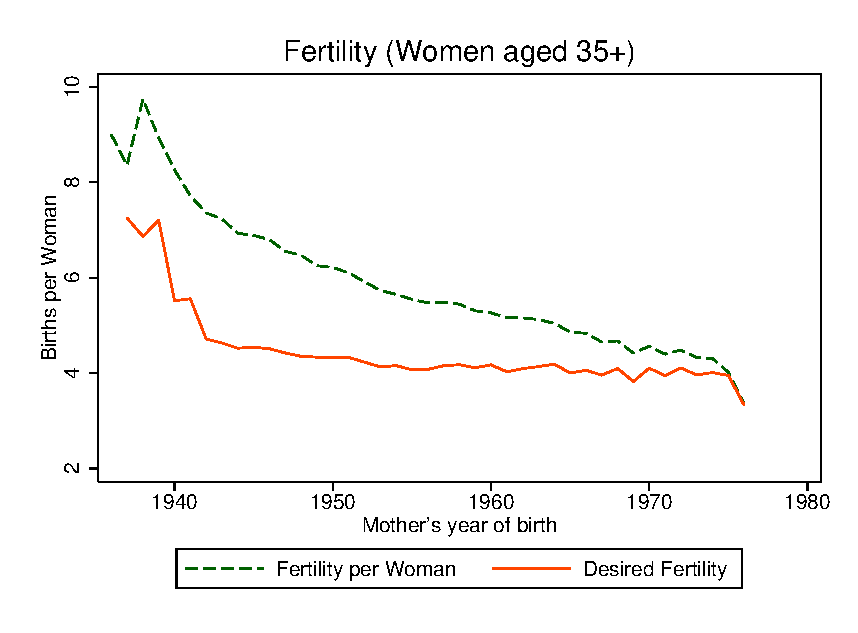
\includegraphics[scale=0.53]{\twinfolder/Figures/ferttrend_35_all.eps}
  \caption{Trends in Fertility}
  \label{TWINfig:fertrend}
\end{subfigure}%
\begin{subfigure}{.5\textwidth}
  \centering
  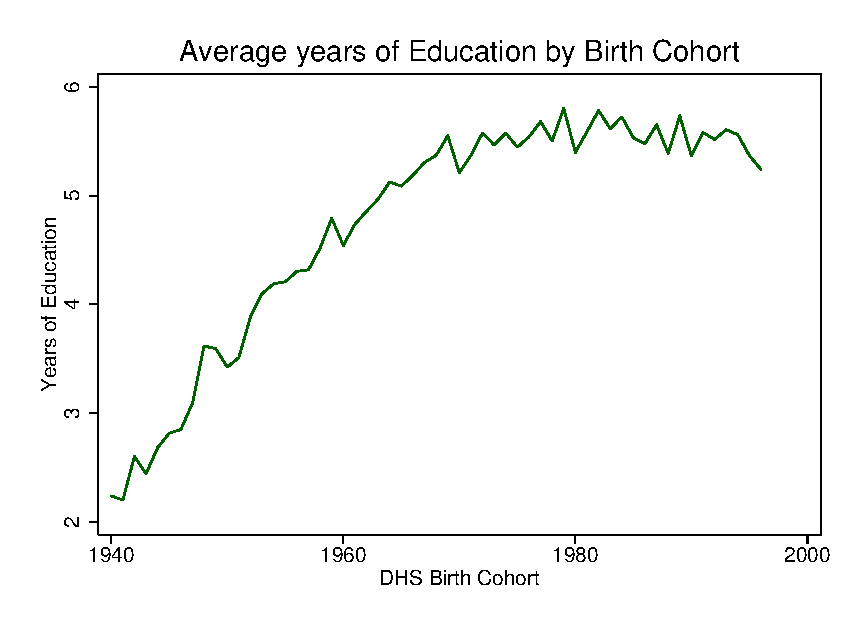
\includegraphics[scale=0.52]{\twinfolder/Figures/eductrend_all.eps}
  \caption{Trend in Education}
  \label{TWINfig:eductrend}
\end{subfigure}
\caption{Education and Fertility}
\label{TWINfig:trends}
\floatfoot{Note to figure \ref{TWINfig:trends}: Cohorts are made up of all individuals 
from the DHS who are over 35 years (for fertility), and over 15 years (for education).  
In each case the sample is restricted to those who have approximately completed fertility 
and education respectively.}
\end{figure}
\vspace{1cm}

\begin{figure}[htpb!]
\begin{center}
\caption{Proportion of Twins of All Births (USA)}
\label{TWINfig:bord}
\includegraphics[scale=0.92]{\twinfolder/Figures/USTwinFLE.eps} 
\end{center}
\end{figure}

\begin{figure}[htpb!]
\begin{center}
\caption{Twin Births and Total Fertility}
\label{TWINfig:births}
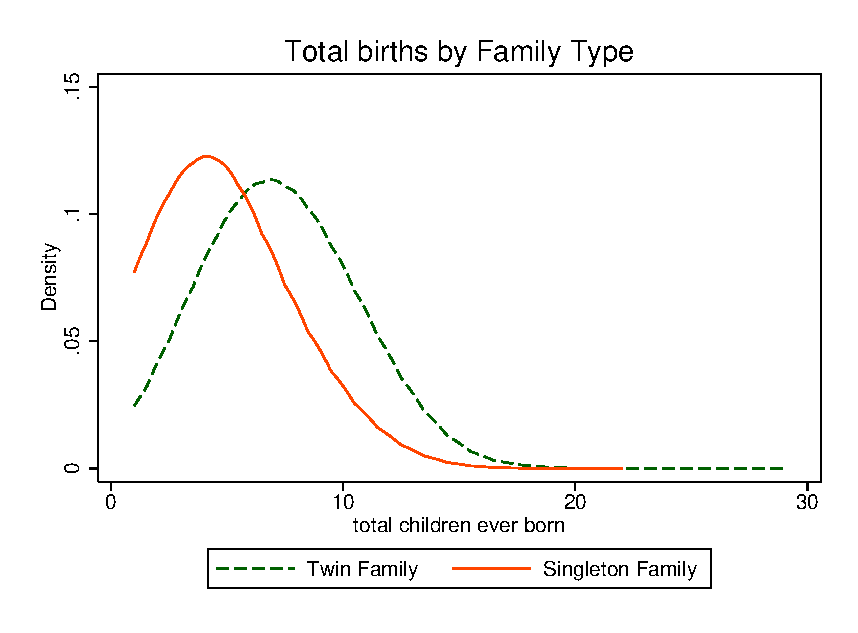
\includegraphics[scale=0.92]{\twinfolder/Figures/famsize.eps} 
\end{center}
\end{figure}

\begin{figure}[htpb!]
\begin{center}
\caption{Proportion of Twins by Birth Order}
\label{TWINfig:bord}
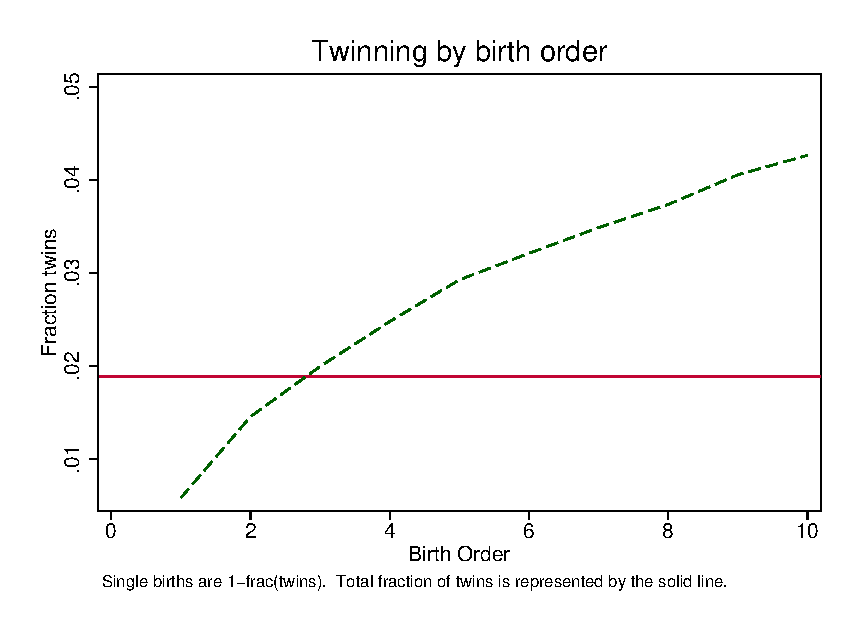
\includegraphics[scale=0.92]{\twinfolder/Figures/twinbybord.eps} 
\end{center}
\end{figure}

\begin{figure}[htpb!]
\begin{center}
\caption{Intra- and Inter-country trends: height and twinning}
\label{TWINfig:arrows}
\includegraphics[scale=0.86]{\twinfolder/Figures/height_country.eps} 
\end{center}
\end{figure}

%\begin{figure}[htpb!]
%\begin{center}
%\caption{Distribution of Ideal Family Size}
%\label{TWINfig:ideal}
%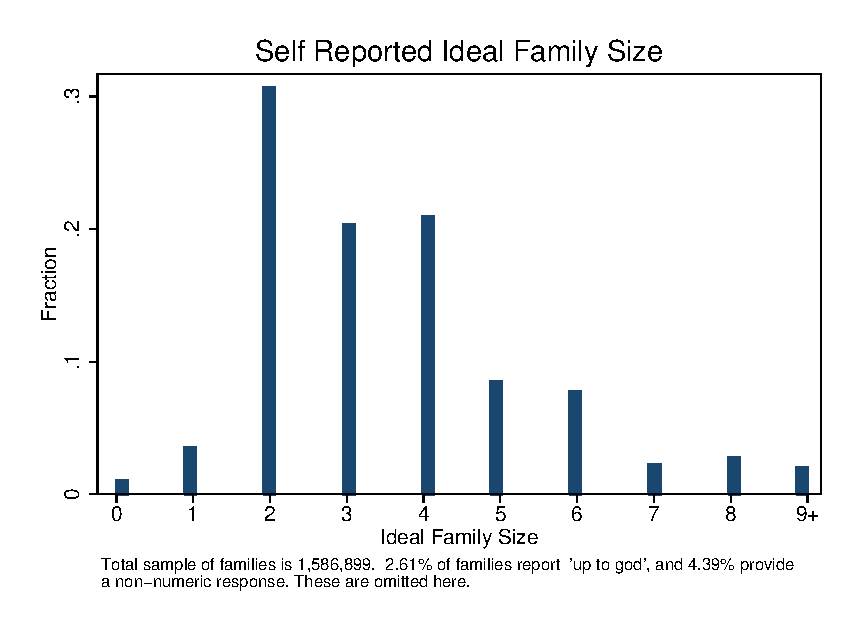
\includegraphics[scale=0.92]{\twinfolder/Figures/idealfamsize.eps} 
%\end{center}
%\end{figure}

%\begin{figure}[htpb!]
%\begin{center}
%\caption{Ideal and Actual Fertility}
%\label{TWINfig:idealactual}
%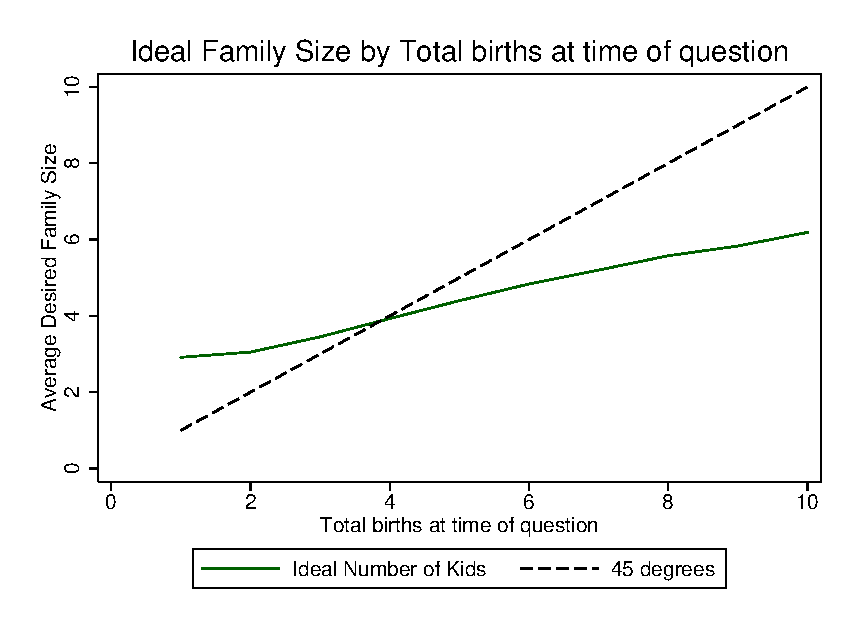
\includegraphics[scale=0.92]{\twinfolder/Figures/idealfam_fert.eps} 
%\end{center}
%\end{figure}

\begin{figure}[htpb!]
\begin{center}
\caption{Relaxing Strict Exogeneity (two plus)}
\label{TWINfig:ltz2}
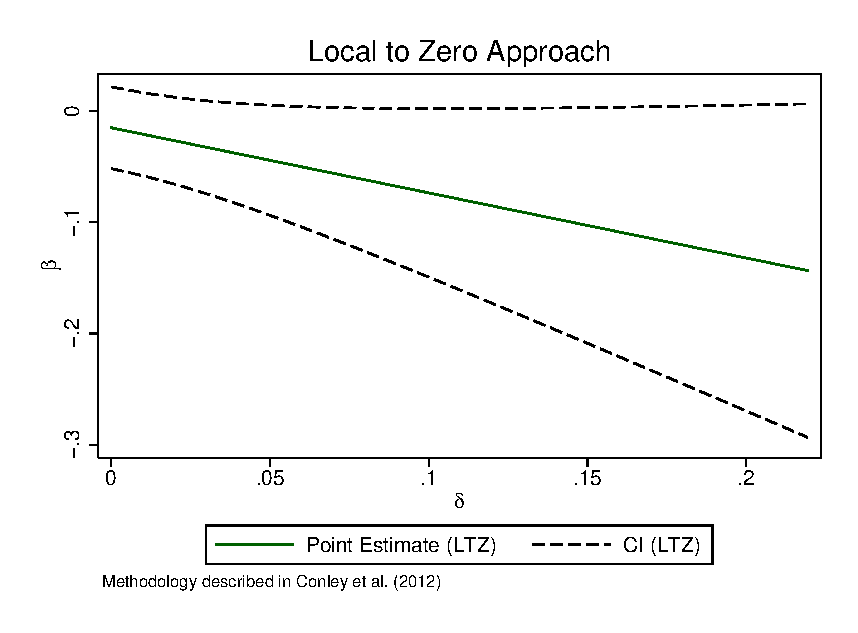
\includegraphics[scale=0.88]{\twinfolder/Figures/LTZ_two.eps}
\vspace{-8mm}
\floatfoot{Note to figure \ref{TWINfig:ltz2}: See note to Figure \ref{TWINfig:ltz3}}
\end{center}
\end{figure}

\begin{figure}[htpb!]
\begin{center}
\caption{Relaxing Strict Exogeneity (three plus)}
\label{TWINfig:ltz3}
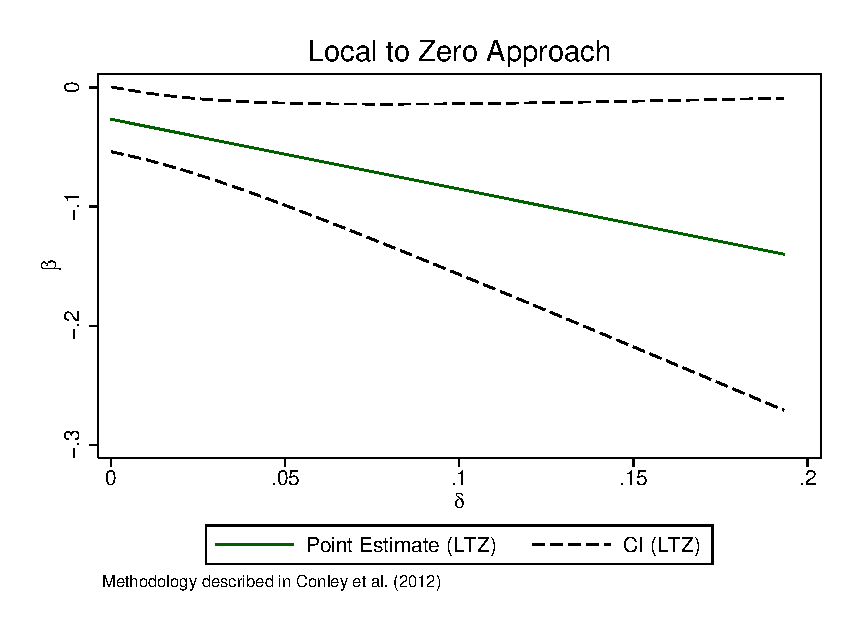
\includegraphics[scale=0.88]{\twinfolder/Figures/LTZ_three.eps} 
\floatfoot{Note to figure \ref{TWINfig:ltz3}: Confidence intervals and point estimates 
are calculated according to \citet{Conleyetal2012}.  Estimates reflect a range of priors 
regarding the validity of the exclusion restriction required to consistently estimate 
$\hat\beta_{fert}$ using twinning in a 2SLS framework.  The local to zero (LTZ) 
approach applied here assumes that $\gamma$, the sign on the instrument when included
in the first stage, is distributed $\gamma\sim U(0,\delta)$.  Further discussion 
is provided in the body of the text and table \ref{TWINtab:Conley}.}
\end{center}
\end{figure}




\clearpage
\section*{Tables}
\input{\twinfolder/Tables/SummaryStatistics.tex}
\clearpage
\input{\twinfolder/Tables/twinEffectsUncond.tex}
\clearpage
\input{\twinfolder/Tables/Stress.tex}
\begin{table}[htpb!]
\caption{Test of hypothesis that women who bear twins have better prior health}\label{TWINtab:IMR}\begin{center}\begin{tabular}{lccc}
\toprule \toprule 
\textsc{Infant Mortality (per 100 births)}& Base & +S\&H & Observations \\ \midrule 
\begin{footnotesize}\end{footnotesize}& 
\begin{footnotesize}\end{footnotesize}& 
\begin{footnotesize}\end{footnotesize}& 
\begin{footnotesize}\end{footnotesize}\\ 
Treated (2+)\hspace{5mm}\hspace{5mm}\hspace{5mm}\hspace{5mm}\hspace{5mm}\hspace{5mm}&-2.065***&-2.110***&503785\\
&(0.212)&(0.213)&\\
Treated (3+)\hspace{5mm}&-4.619***&-4.632***&686931\\
&(0.201)&(0.201)&\\
Treated (4+)&-4.257***&-4.243***&676303\\
&(0.183)&(0.183)&\\
Treated (5+)&-3.353***&-3.324***&587919\\
&(0.183)&(0.183)&\\
\midrule\multicolumn{4}{p{12.1cm}}{\begin{footnotesize}\textsc{Notes:} The sample for these regressions consist of all children who have been entirely exposed to the risk of infant mortality (ie those over 1 year of age). Subsamples 2+, 3+, 4+ and 5+ are generated to allow comparison of children born at similar birth orders.  For a full description of these groups see the the body of the paper or notes to table \ref{TWINtab:IVAll}. Treated=1 refers to children who are born before a twin while Treated=0 refers to children of similar birth orders not born before a twin.  Base and S+H controls are described in table \ref{TWINtab:IVAll}.$^{*}$p$<$0.1; $^{**}$p$<$0.05; $^{***}$p$<$0.01 
\end{footnotesize}} \\ \bottomrule 
\end{tabular}\end{center}\end{table}


\input{\twinfolder/Tables/Alderman.tex}
\begin{landscape}
\input{\twinfolder/Tables/FDeath_Uncond.tex}
\end{landscape}
\input{\twinfolder/Tables/DHS-NHIS-OLS.tex}
\input{\twinfolder/Tables/DHS-togetherIV.tex}
\input{\twinfolder/Tables/NHIS-togetherIV.tex}
\input{\twinfolder/Tables/gamma.tex}
\begin{table}[htpb!]\caption{`Plausibly Exogenous' Bounds} 
\label{TWINtab:Conley}\begin{center}\begin{tabular}{lcccc}
\toprule \toprule 
&\multicolumn{2}{c}{UCI: $\gamma\in [0,\delta]$}&\multicolumn{2}{c}{LTZ: $\gamma \sim U(0,\delta)$}\\ 
\cmidrule(r){2-3} \cmidrule(r){4-5}
&Lower Bound&Upper Bound&Lower Bound&Upper Bound\\
Two Plus&-0.1860&0.0195&-0.1613&0.0011\\
Three Plus&-0.1710&0.0025&-0.1528&-0.0116\\
Four Plus&-0.1539&-0.0067&-0.1391&-0.0194\\
Five Plus&-0.1373&0.0277&-0.1215&0.0143\\
\midrule\multicolumn{5}{p{11.6cm}}{\begin{footnotesize}\textsc{Notes:} This table presents upper and lower bounds of a 95\% confidence interval for the effects of family size on (standardised) children's education attainment. These are estimated by the methodology of \citet{Conleyetal2012}  under various priors about the direct effect that being from a twin family has on educational outcomes ($\gamma$). In the UCI (union of confidence interval) approach, it is assumed the true $\gamma\in[0,\delta]$, while in the LTZ (local to zero) approach it is assumed that $\gamma\sim U(0,\delta)$.  In each case $\delta$ is estimated by including twinning in the first stage  equation and observing the effect size $\hat\gamma$.  Estimated $\hat\gamma$'s are (respectively for two plus to five plus):   0.1088, 0.0983, 0.0826, 0.0929.\end{footnotesize}}  
\\ \bottomrule \end{tabular}\end{center}\end{table} 

\clearpage


\bibliography{./BiBBase1}

\end{spacing}
\end{document}
